



%----------------------------------------------------------------------------------------

\newpage

%%%%%%%%%%%%%%%%%%%%%%%
\section{Network generation heuristics}{Heuristiques de génération de réseau}

\label{app:sec:networkgrowth}



%%%%%%%%%%%%%%%%%%%%%%%
\subsection{Slime mould model}{Modèle de slime mould}


\bpar{
We recall here the procedure of type \emph{slime mould} to evolve the biological network, based on~\cite{tero2007mathematical}. The network is composed by nodes characterized by their pressure $p_i$ and by links characterized by their length $L_{ij}$, their diameter $D_{ij}$, an impedance $Z_{ij}$ and the flow traversing them $\phi_{ij}$. The relation analogous to Ohm's law for links writes
}{
Nous rappelons ici la procédure d'évolution du réseau biologique de type \emph{slime mould}, à partir de~\cite{tero2007mathematical}. Le réseau est composé de noeuds caractérisés par leur pression $p_i$ et de liens caractérisés par leur longueur $L_{ij}$, leur diamètre $D_{ij}$, une impédance $Z_{ij}$ et le flux les traversant $\phi_{ij}$. La relation analogue à la loi d'Ohm pour les liens s'écrit
}

\[
\phi_{ij} = \frac{D_{ij}}{Z_{ij}\cdot L_{ij}} \left(p_i - p_j\right)
\]

\bpar{
Furthermore, the conservation of flows at each node (Kirchoff's law) imposes
}{
Par ailleurs, la conservation des flux à chaque noeud (loi de Kirchoff) impose
}

\[
\sum_i \phi_{ij} = 0
\]

\bpar{
for all $j$ except the source and the sink, that we assume at indices $j_+$ and $j_-$, such that $\sum_i \phi_{ij_+} = I_0$ and $\sum_i \phi_{ij_-} = -I_0$ with $I_0$ initial flow parameter.
}{
pour tout $j$ sauf pour la source et le puit, que nous supposons aux indices $j_+$ et $j_-$, tel que $\sum_i \phi_{ij_+} = I_0$ et $\sum_i \phi_{ij_-} = -I_0$ avec $I_0$ paramètre de flux initial.
}

\bpar{
The combination of above constraints gives for all $j$
}{
La combinaison des contraintes ci-dessus donne pour tout $j$
}

\[
\sum_i \frac{D_{ij}}{Z_{ij}\cdot L_{ij}} (p_i - p_j) = \mathbbm{1}_{j=j_+} I_0 - \mathbbm{1}_{j=j_-} I_0 
\]

\bpar{
what simplifies into a matrix equation, by denoting $\mathbf{Z} = \left(\frac{\frac{D_{ij}}{Z_{ij}\cdot L_{ij}}}{\sum_i \frac{D_{ij}}{Z_{ij}\cdot L_{ij}}}\right)_{ij}$, and also $\vec{k} = \frac{\mathbbm{1}_{j=j_+} I_0 - \mathbbm{1}_{j=j_-} I_0 }{\sum_i \frac{D_{ij}}{Z_{ij}\cdot L_{ij}}}$ and $\vec{p} = p_i$, what simplifies into
}{
ce qui se simplifie en une équation matricielle, en notant $\mathbf{Z} = \left(\frac{\frac{D_{ij}}{Z_{ij}\cdot L_{ij}}}{\sum_i \frac{D_{ij}}{Z_{ij}\cdot L_{ij}}}\right)_{ij}$, ainsi que $\vec{k} = \frac{\mathbbm{1}_{j=j_+} I_0 - \mathbbm{1}_{j=j_-} I_0 }{\sum_i \frac{D_{ij}}{Z_{ij}\cdot L_{ij}}}$ et $\vec{p} = p_i$, qui se simplifie en
}

\[
\left(Id - \mathbf{Z}\right) \vec{p} = \vec{k}
\]


\bpar{
The system admits a solution when $\left(Id - \mathbf{Z}\right)$ is invertible. The space of invertible matrices being dense in $\mathcal{M}_n(\mathbb{R})$, by multilinearity of the determinant, an infinitesimal perturbation of the position of nodes allows to invert the matrix if it is indeed singular. We obtain thus the pressures $p_i$ and as a consequence the flows $\phi_{ij}$.
}{
Le système admet une solution lorsque $\left(Id - \mathbf{Z}\right)$ est inversible. L'espace des matrices inversible étant dense dans $\mathcal{M}_n(\mathbb{R})$, par multilinéarité du déterminant, une perturbation infinitésimale de la position des noeuds permet d'inverser la matrice si celle-ci est effectivement singulière. On obtient donc les pressions $p_i$ et par conséquent les flux $\phi_{ij}$.
}

% François le resoud avec https://arxiv.org/pdf/1301.6628.pdf
% https://github.com/fqueyroi/tulip_plugins/blob/master/TransportationNetworks/FlowBetweenness/flowbetweenness.cpp


\bpar{
The evolution of the diameter $D_{ij}$ between two equilibrium stages is a function of the flow at equilibrium, through the equation
}{
L'évolution du diamètre $D_{ij}$ entre deux étapes d'équilibre est fonction du flux à l'équilibre, par l'équation 
}

\[
D_{ij} (t+1) - D_{ij} = \delta t \left[ \frac{\phi_{ij}(t)^\gamma}{1 + \phi_{ij}(t)^\gamma} - D_{ij}(t)\right]
\]

\bpar{
We take to simplify $\gamma = 1.8$, following the configuration used by~\cite{tero2010rules} for the generation of a network in a real configuration. We furthermore take $\delta t = 0.05$ and $I_0 = 10$.
}{
Nous prenons pour simplifier $\gamma = 1.8$, suivant la configuration utilisée par~\cite{tero2010rules} pour la génération d'un réseau dans une configuration réelle. Nous prenons par ailleurs $\delta t = 0.05$ et $I_0 = 10$.
}

\bpar{
The generation of a network can be achieved from an initial network, until reaching a convergence criteria, for example $\sum_{ij} \Delta D_{ij} (t) < \varepsilon$ with $\varepsilon$ fixed threshold parameter. We will use this model with a criteria of a number of iterations, and proceed to an iteration to obtain final networks with a reasonable number of links.
}{
La génération d'un réseau peut s'effectuer à partir d'un réseau initial, jusqu'à atteindre un critère de convergence, par exemple $\sum_{ij} \Delta D_{ij} (t) < \varepsilon$ avec $\varepsilon$ paramètre de seuil fixé. Nous utilisons ce modèle avec un critère de nombre d'itérations, et procédons à une itération pour obtenir des réseaux finaux avec un nombre raisonnable de liens.
}




%%%%%%%%%%%%%%%%%%%%%%%
\subsection{Results}{Résultats}


\bpar{
In the experiment exploring the distance to real networks, the initialization of the density is done according to 50 density grids classified into 5 morphological classes (10 grids per class). The Table~\ref{app:tab:networkgrowth:morpho} gives the composition of centers of classes in terms of morphological indicators. Classes can be interpreted the following way:
\begin{itemize}
	\item Class 5: lowest Moran, high distance, hierarchy and entropy; numerous population centers that are localized and dispersed.
	\item Class 4: highest entropy and hierarchy; a small number of localized centers.
	\item Class 3: lowest distance and entropy; diffuse population.
	\item Class 2: highest Moran; one or a few centers with consequent size.
	\item Class 1: intermediate values for all indicators; a certain number of centers of intermediate size.
\end{itemize}
}{
Dans l'expérience explorant la distance aux réseaux réels, l'initialisation de la densité est faite selon 50 grilles classées dans 5 classes morphologiques (10 grilles par classe). La Table~\ref{app:tab:networkgrowth:morpho} donne la composition des centres des classes en termes d'indicateurs morphologiques. Les classes peuvent être interprétées de la façon suivante :
\begin{itemize}
	\item Classe 5 : plus bas Moran, distance, hiérarchie et entropie élevées ; nombreux foyers de peuplement localisés et dispersés.
	\item Classe 4 : plus fortes entropie et hiérarchie ; un petit nombre de foyers localisés.
	\item Classe 3 : plus basse distance et entropie ; population diffuse.
	\item Classe 2 : plus haut Moran ; un ou quelques centres de taille conséquente.
	\item Classe 1 : valeurs intermédiaires pour tous les indicateurs ; un certain nombre de centres de taille intermédiaire.
\end{itemize}
}


%%%%%%%%%%%%%%%
\begin{table}
\apptabcaption{\textbf{Morphological indicators for centers of classes for initial density grids.}\label{app:tab:networkgrowth:morpho}}{\textbf{Indicateurs morphologiques pour les centres des classes des grilles de densité initiales.}\label{app:tab:networkgrowth:morpho}}
\begin{tabular}{|c|c|c|c|c|}
\hline
\bpar{
Class & Moran $I$ & Distance $\bar{d}$ & Entropy $\mathcal{E}$ & Hierarchy $\gamma$ \\\hline 
}{
Classe & Moran $I$ & Distance $\bar{d}$ & Entropie $\mathcal{E}$ & Hiérarchie $\gamma$ \\\hline 
}
1 & 0.23 & 0.66 & 0.76 & 0.62 \\\hline % medium everything
2 & 0.47 & 0.50 & 0.75 & 0.53 \\\hline % highest moran, medium others
3 & 0.21 & 0.42 & 0.57 & 0.65 \\\hline % lowest distance and entropy, medium slope
4 & 0.24 & 0.75 & 0.90 & 0.87 \\\hline % highest entropy and slope
5 & 0.15 & 0.76 & 0.84 & 0.72 \\\hline % lowest moran, high distance, slope and entropy
\end{tabular}
\end{table}
%%%%%%%%%%%%%%%


\bpar{
Topological spaces of networks generated in~\ref{sec:networkgrowth} can be conditioned to morphological classes for initial density distribution. This conditioning is shown in Fig.~\ref{fig:app:networkgrowth:feasiblespace_bymorph}. We also give feasible spaces with real points. Classes 1 and 5 seem to be the ones for which being close to real points is the easiest, in terms of extreme points.
}{
Les espaces topologiques des réseaux générés en~\ref{sec:networkgrowth} peuvent être conditionnés aux classes morphologiques pour la distribution de densité initiale. Ce conditionnement est montré en Fig.~\ref{fig:app:networkgrowth:feasiblespace_bymorph}. Nous donnons également les espaces faisables avec les points réels. Les classes 1 et 5 semblent être celles pour laquelle le rapprochement aux points réels est le plus facile, en termes de points extrêmes.
}


%%%%%%%%%%%%%%%%%
\begin{figure}
%\includegraphics[width=\linewidth]{Figures/NetworkGrowth/feasible_space_pca_bymorph}
%\includegraphics[width=\linewidth]{Figures/NetworkGrowth/feasible_space_withreal_pca_bymorph}
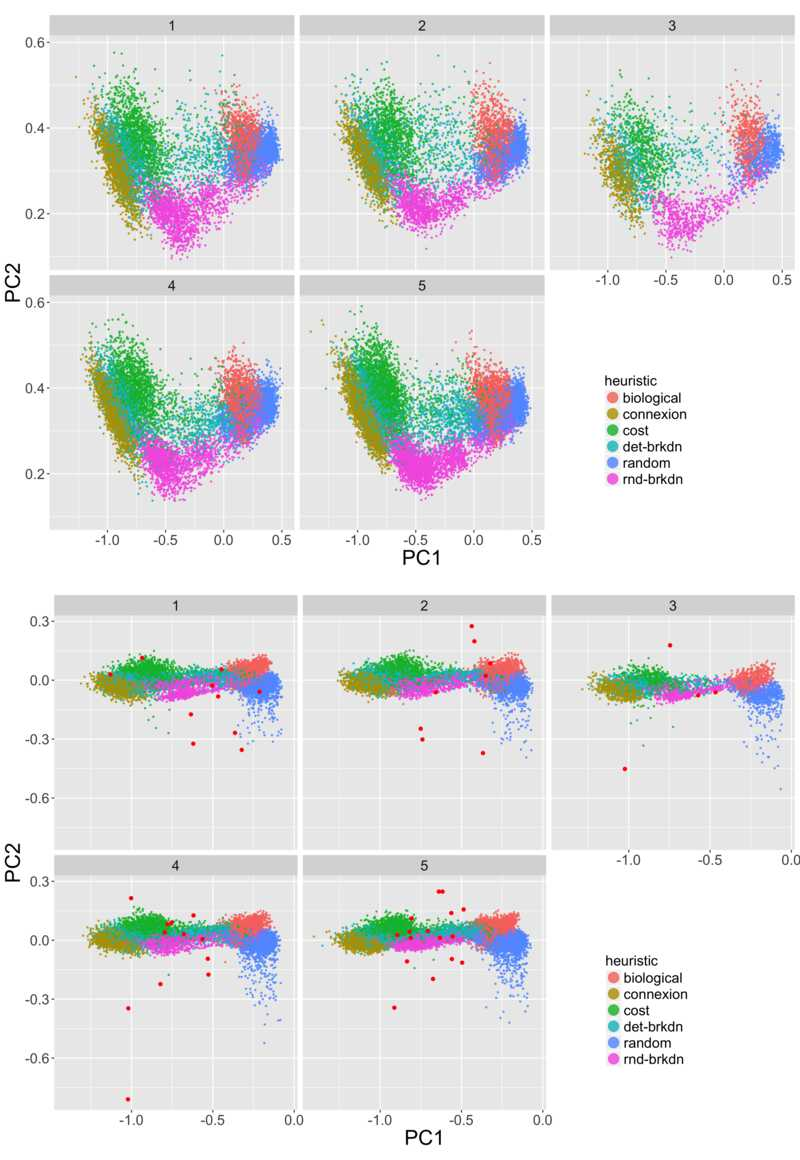
\includegraphics[width=0.9\linewidth]{Figures/Final/A-networkgrowth-feasiblespace_bymorph}
\appcaption{\textbf{Conditioning of results to morphological classes for density.} (\textit{Top}) Topological feasible space for the different generation heuristics, conditioned to the morphological density class. (\textit{Bottom}) Same plots with real points in red.\label{fig:app:networkgrowth:feasiblespace_bymorph}}{\textbf{Conditionnement des résultats aux classes morphologiques pour la densité.} (\textit{Haut}) Espace topologique faisable pour les différentes heuristiques de génération, conditionné à la classe morphologique de densité. (\textit{Bas}) Mêmes graphiques avec les points réels en rouge.\label{fig:app:networkgrowth:feasiblespace_bymorph}}
\end{figure}
%%%%%%%%%%%%%%%%%









%----------------------------------------------------------------------------------------

\newpage

%%%%%%%%%%%%%%%%%%%%%%%
\section{Co-evolution at the mesoscopic scale}{Co-évolution à l'échelle mesoscopique}

\label{app:sec:mesocoevolmodel}


%%%%%%%%%%%%%%%%%%%%%%%
\subsection{Calibration}{Calibration}


\bpar{
In order to justofy the aggregation of distances for indicators and for correlations, we have visually controlled the shape of Pareto fronts for these two objectives for around twenty simulated points. An example for two points is given in Fig.~\ref{fig:app:mesocoevolmodel:paretodists}. It appears that these fronts are close to be not existing, i.e. that there almost exist a global optimum.
}{
Afin de justifier l'agrégation des distances pour les indicateurs et pour les corrélations, nous avons contrôlé visuellement la forme des fronts de Pareto pour ces deux objectifs pour une vingtaine de points simulés. Un example pour deux points est donné en Fig.~\ref{fig:app:mesocoevolmodel:paretodists}. Il apparait que ces fronts sont quasi-inexistants, c'est-à-dire qu'il existe presque un optimum global.
}


\bpar{
Let illustrate to what extent a linear aggregation with equal coefficients can be relevant in the case of a Pareto front which is close to being vertical/horizontal. The function
}{
Illustrons dans quelle mesure une agrégation linéaire à coefficient égaux peut être pertinente dans le cas d'un front de Pareto quasiment vertical/horizontal. La fonction
}
\[
f_{\alpha} : x \mapsto \frac{1}{(x+1)^\alpha}
\]
\bpar{
takes this form in a neighborhood of 0 when $\alpha$ becomes large. We then consider the two objectives $o_1(x) = x$ and $o_2(x) = f_{\alpha}(x)$, which can either be considered for a bi-objective minimization, or in the frame of a linear aggregation through the minimization of $o(x) = \beta x + (1-\beta) \frac{1}{(x+1)^{\alpha}}$. That latest is minimal in $x = \left(\frac{\beta}{\alpha (1-\beta)}\right)^{\frac{1}{\alpha + 1}} - 1$, term which can be developed into
}{
prend cette forme dans un voisinage de 0 lorsque $\alpha$ devient grand. Considérons alors les deux objectifs $o_1(x) = x$ et $o_2(x) = f_{\alpha}(x)$, qui peuvent soit être considérés pour une minimisation bi-objectifs, soit dans le cadre d'une agrégation linéaire par minimisation de $o(x) = \beta x + (1-\beta) \frac{1}{(x+1)^{\alpha}}$. Cette dernière est minimale en $x = \left(\frac{\beta}{\alpha (1-\beta)}\right)^{\frac{1}{\alpha + 1}} - 1$, terme qui se développe en 
}
\[
x = \frac{\ln\left(\beta (1-\beta)\right)}{\alpha + 1} + \frac{\ln\alpha}{\alpha + 1} + o(\frac{1}{\alpha})
\]

\bpar{
Furthermore, let consider that in the frame of a bi-objective optimization, we take the compromise at which the variations of $o_1$ equalize the ones of $o_2$, what is equivalent to take $x$ such that $\frac{\partial f}{\partial x} = \frac{\partial f^{-1}}{\partial x}$. This equation leads to $\frac{x^{\frac{1}{\alpha}}}{x + 1} = \frac{1}{\alpha^{\frac{2}{\alpha + 1}}}$. We can then develop at the second order on each side to obtain
}{
Par ailleurs, considérons que dans le cadre d'une optimisation bi-objectifs, nous prenions le compromis auquel les variations de $o_1$ égalent celles de $o_2$, ce qui revient à prendre $x$ tel que $\frac{\partial f}{\partial x} = \frac{\partial f^{-1}}{\partial x}$. Cette équation conduit à $\frac{x^{\frac{1}{\alpha}}}{x + 1} = \frac{1}{\alpha^{\frac{2}{\alpha + 1}}}$. On peut alors développer au second ordre de chaque côté pour obtenir
}
\[
\frac{\ln x}{\alpha} = x \left[1 - 2 \frac{\ln \alpha}{\alpha + 1} + o(\frac{1}{\alpha})\right] - 2 \frac{\ln \alpha}{\alpha + 1} + o(\frac{1}{\alpha}) 
\]
\bpar{
We indeed necessarily have $x\rightarrow_{\alpha \rightarrow \infty} 0$, since if $x \rightarrow K \neq 0$, we have a contradiction in the previous equation since $1/(1+K) \neq 0$. It implies that $\frac{\ln x}{\alpha} = o(\frac{1}{\alpha})$, and thus that
}{
Or on a nécessairement $x\rightarrow_{\alpha \rightarrow \infty} 0$, puisque si $x \rightarrow K \neq 0$, on a une contradiction dans l'équation précédente car $1/(1+K) \neq 0$. Cela implique que $\frac{\ln x}{\alpha} = o(\frac{1}{\alpha})$, et donc que
}
\[
x = 2 \frac{\ln \alpha}{\alpha + 1} + o(\frac{1}{\alpha})
\]
\bpar{
In order thus to have the same order of magnitude for the solutions to the two approaches, we need to eliminate the term in $1/(\alpha + 1)$ in the first, what is equivalent to take $\ln \left(\beta (1- \beta)\right) = 0$ and therefore $\beta = 1/2$.
}{
Pour avoir donc les mêmes ordres de grandeur pour les solutions aux deux approches, il faut éliminer le terme en $1/(\alpha + 1)$ dans la première, ce qui revient à prendre $\ln \left(\beta (1- \beta)\right) = 0$ et donc $\beta = 1/2$.
}

\bpar{
Thus, there is equivalence of orders of magnitude in $\alpha$ for the two approaches if an only if $\beta = 1/2$. Given the shape of our Pareto fronts, we consider that the solution is analogous and consider thus the sum of the two distances.
}{
Ainsi, il y a équivalence des ordres de grandeurs en $\alpha$ pour les deux approches si et seulement si $\beta = 1/2$. Vu la forme de nos fronts de Pareto, nous considérons la solution analogue et considérons ainsi la somme des deux distances.
}


%%%%%%%%%%%%%%
\begin{figure}
	%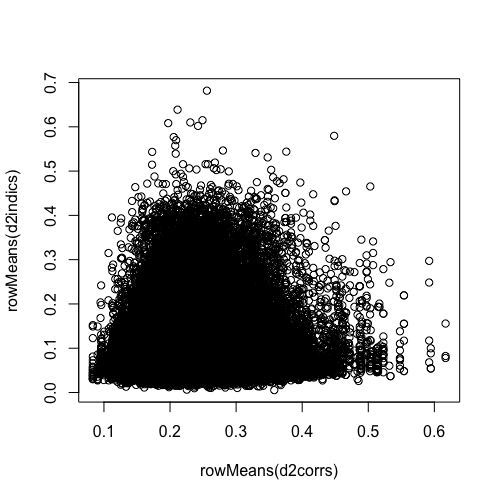
\includegraphics[width=0.49\linewidth]{Figures/MesoCoEvol/dists_pareto_i1.png}
	%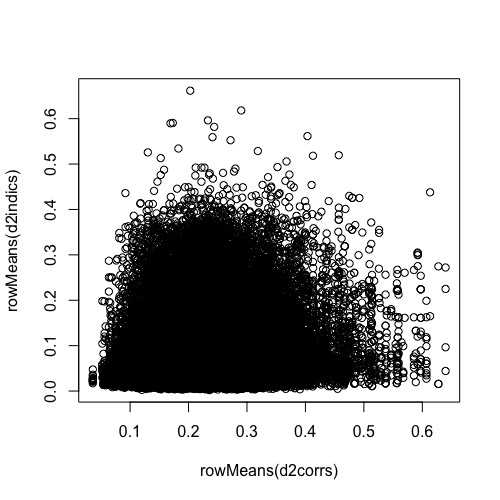
\includegraphics[width=0.49\linewidth]{Figures/MesoCoEvol/dists_pareto_i10.png}
	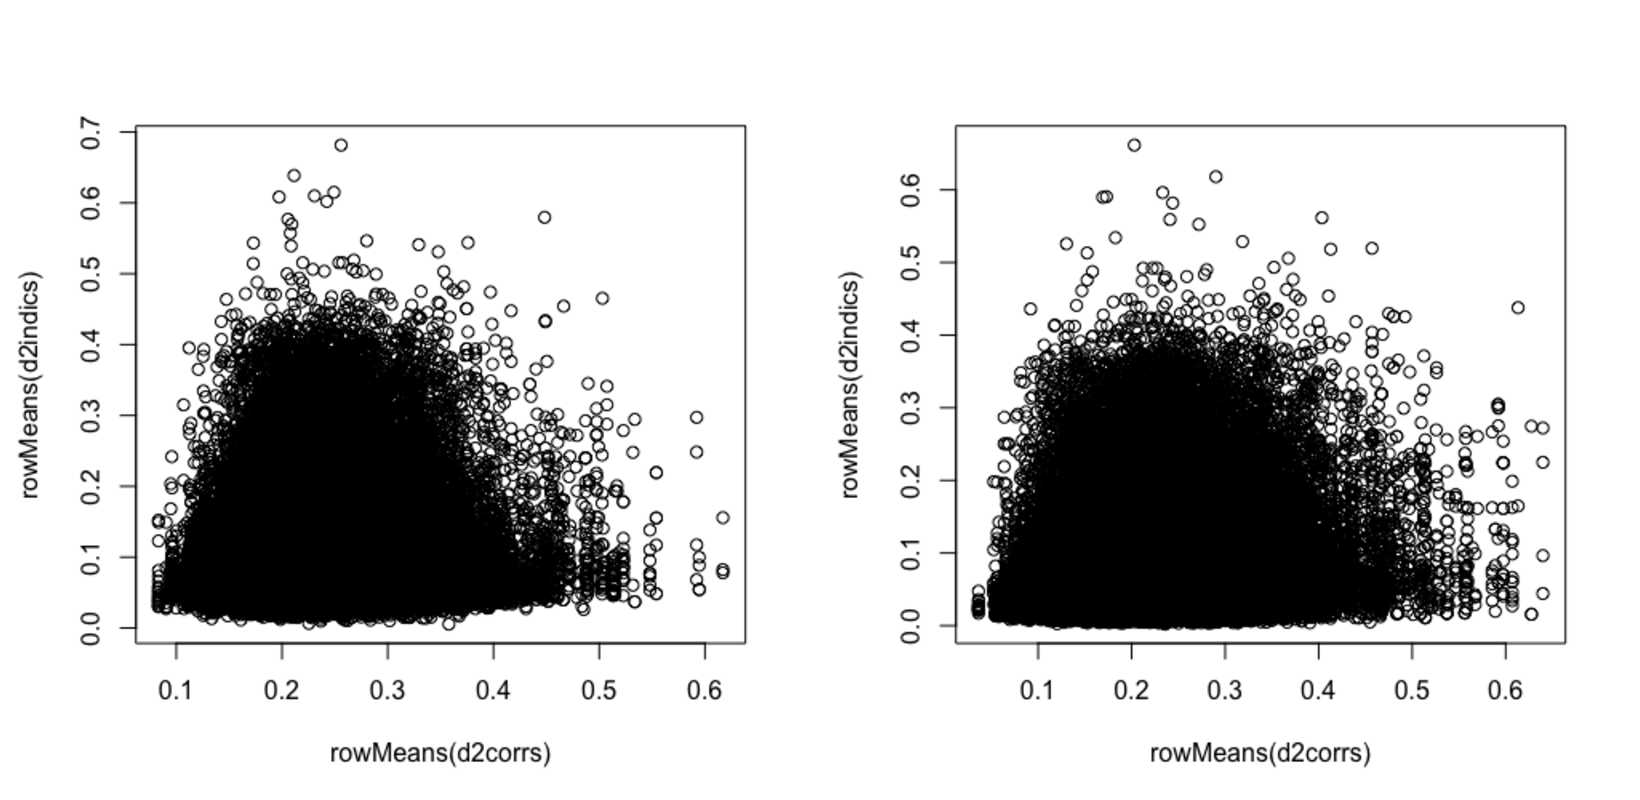
\includegraphics[width=\linewidth]{Figures/Final/A-mesocoevolmodel-paretodists.jpg}
	\appcaption{\textbf{Example of Pareto fronts for the calibration at the first and second order.} We give for two particular simulation points, the distances to indicators $d_I^2$ and the distances to correlations $d_C^2$ for all the real points.\label{fig:app:mesocoevolmodel:paretodists}}{\textbf{Exemples de fronts de Pareto pour la calibration au premier et au second ordre.} Nous donnons pour deux points particuliers de simulation, les distances aux indicateurs $d_I^2$ et les distances aux corrélations $d_C^2$ pour l'ensemble des points réels.\label{fig:app:mesocoevolmodel:paretodists}}
\end{figure}
%%%%%%%%%%%%%%







%----------------------------------------------------------------------------------------

\newpage

%%%%%%%%%%%%%%%%%%%%%%%
\section{Transportation system governance modeling}{Modélisation de la gouvernance du système de transport}

\label{app:sec:lutecia}


%%%%%%%%%%%%%%%%%%%%%%%
\subsection{Land-use model}{Modèle d'usage du sol}


\subsubsection{Convergence}{Convergence}

\bpar{
We study here the issue of the convergence in time of the distribution of activities, with a fixed infrastructure.
}{
Nous étudions ici la question de la convergence dans le temps de la distribution des activités, à infrastructure fixe.
}

\bpar{
Let consider a very simple case: by taking $\lambda = 0$ the problem is made not spatial and by taking $\gamma_A = 1$ we achieve the decoupling between population and employments. By denoting $\beta' = \sum_j E_j \cdot \beta$ and $P_0 = \alpha \cdot \sum_i P_i$, the existence of a fixed point for populations is equivalent to the resolution of
}{
Considérons un cas très simple : en prenant $\lambda = 0$ on déspatialise le problème et en prenant $\gamma_A = 1$ on finit de découpler population et emplois. En posant $\beta' = \sum_j E_j \cdot \beta$ et $P_0 = \alpha \cdot \sum_i P_i$, l'existence d'un point fixe pour les populations se ramène à la résolution de
}
\[
P_i = P_0 \cdot \frac{\exp\left(\beta' \cdot P_i\right)}{\sum \exp\left(\beta' \cdot P_i\right)}
\]

\bpar{
The function is indeed continuous in $P_i$ and variation ranges for population are $[0,\sum_i P_i]$, it therefore admits a fixed point through the Brouwer fixed point theorem.
}{
La fonction est bien continue en les $P_i$ et les plages de variations de la population sont $[0,\sum_i P_i]$, elle admet donc un point fixe par le Théorème du Point Fixe de Brouwer. 
}

\bpar{
Indeed, in all generality, if we write
}{
En fait, en toute généralité, si on écrit
}

\[
(\vec{P}(t+1),\vec{E}(t+1)) = f(\vec{P}(t),\vec{E}(t))
\]

\bpar{
for arbitrary parameter values, the function $f$ is also continuous in each component, and takes its values with a bounded closed interval (employments being also limited) therefore a compact. The same way that \cite{leurent2014user} establishes it for a model of traffic flows, we also have a fixed point in our case, what corresponds to an equilibrium point. The unicity is however not trivial and there is no reason for it to be a priori verified. We empirically verify the systematic convergence at fixed infrastructure (see below the exploration of the parameter space).
}{
pour des valeurs des paramètres arbitraires, la fonction $f$ est également continue en chaque composante, et prend ses valeurs dans un fermé borné (les emplois étant également limités) donc compact. De la même manière que \cite{leurent2014user} l'établit pour un modèle de flux de traffic, on a aussi un point fixe dans notre cas, ce qui correspond à un point d'équilibre. L'unicité n'est cependant pas triviale et il n'y a pas de raison qu'elle soit vérifiée a priori. On vérifie empiriquement la convergence systématique à infrastructure fixe (voir ci-dessous l'exploration de l'espace des paramètres).
}

\subsubsection{Exploration}{Exploration}


\bpar{
We proceed to an exploration of the behavior of the land-use model alone, i.e. at fixed infrastructure, in order to understand the influence of parameters on the urban form. We fix $\alpha = 1$ here to study the model in an extreme case.
}{
Nous procédons à une exploration du comportement du modèle d'usage du sol seul, i.e. à infrastructure fixe, afin de comprendre l'influence des paramètres sur la forme urbaine. Nous fixons $\alpha = 1$ ici pour étudier le modèle dans un cas extrême.
}

\bpar{
We follow the urban form indicators defined in~\ref{sec:staticcorrelations}, for the distribution of population and employments, in time and until the model has converged. We reduce the morphological space of the spatial distribution of actives in a principal plan, such that $PC_1 = -0.98 \cdot I - 0.13 \cdot \mathcal{E} + 0.05 \bar{d} - 0.13 \cdot \gamma $ and $PC_2 = -0.19 \cdot I + 0.57 \cdot \mathcal{E} - 0.16 \bar{d} + 0.77 \cdot \gamma $. The first component expresses a level of dispersion and the second a hierarchical aggregation.
}{
Nous suivons les indicateurs de forme urbaine définis en~\ref{sec:staticcorrelations}, pour la distribution de la population et pour les emplois, dans le temps et jusqu'après convergence. Nous réduisons l'espace morphologique de la distribution spatiale des actifs dans un plan principal, tel que $PC_1 = -0.98 \cdot I - 0.13 \cdot \mathcal{E} + 0.05 \bar{d} - 0.13 \cdot \gamma $ et $PC_2 = -0.19 \cdot I + 0.57 \cdot \mathcal{E} - 0.16 \bar{d} + 0.77 \cdot \gamma $. La première composante exprime un niveau de dispersion et la seconde une agrégation hiérarchique.
}

% note : we do not explicitely specify the convergence criteria here ?


\bpar{
The Fig.~\ref{fig:app:lutecia:morphotrajs} gives temporal trajectories in the plan $(PC_1,PC_2)$ for $\gamma_A = 0.9$, $\gamma_E = 0.6$, $v_0 = 6$, for different values of $\lambda$ and $\beta$ and also for different initial networks. We observe that increasing $\beta$ has the tendency to make trajectories uniform. For $\beta = 1$, the shape of the network strongly conditions trajectories conjointly to $\lambda$: we switch for example from a decreasing dispersion and a u-shaped hierarchy to a stable dispersion and an increasing hierarchy for low values of $\lambda$, between no network and a spider network. 
}{
La Fig.~\ref{fig:app:lutecia:morphotrajs} donne des trajectoires temporelles dans le plan $(PC_1,PC_2)$ pour $\gamma_A = 0.9$, $\gamma_E = 0.6$, $v_0 = 6$, pour différentes valeurs de $\lambda$ et de $\beta$ ainsi que pour différents réseaux initiaux. On constate qu'augmenter $\beta$ a tendance à uniformiser les trajectoires. Pour $\beta = 1$, la forme du réseau conditionne fortement les trajectoire conjointement à $\lambda$ : on passe par exemple d'une dispersion décroissante et d'une hiérarchie en cloche à une dispersion stable et une hiérarchie croissante pour les valeurs faibles de $\lambda$, entre aucun réseau et un réseau araignée.
}


% morphoActiveTrajs_gammaCDA0.9_gammaCDE0.6
% Morphology
% "PC1" "PC2" "PC3" "PC4"
%"moranActives" -0.980084779269111 -0.195512301926648 -0.0273364571430177 0.0214821635602741
%"entropyActives" -0.137030712105593 0.570339690854727 0.221651600681317 -0.778977399473809
%"meanDistanceActives" 0.0503574253429071 -0.168869841317757 -0.903924010571035 -0.389703078662877
%"slopeActives" -0.134612551783578 0.779724665202014 -0.364752887773974 0.490779215369261



%%%%%%%%%%%%%%
\begin{figure}
	%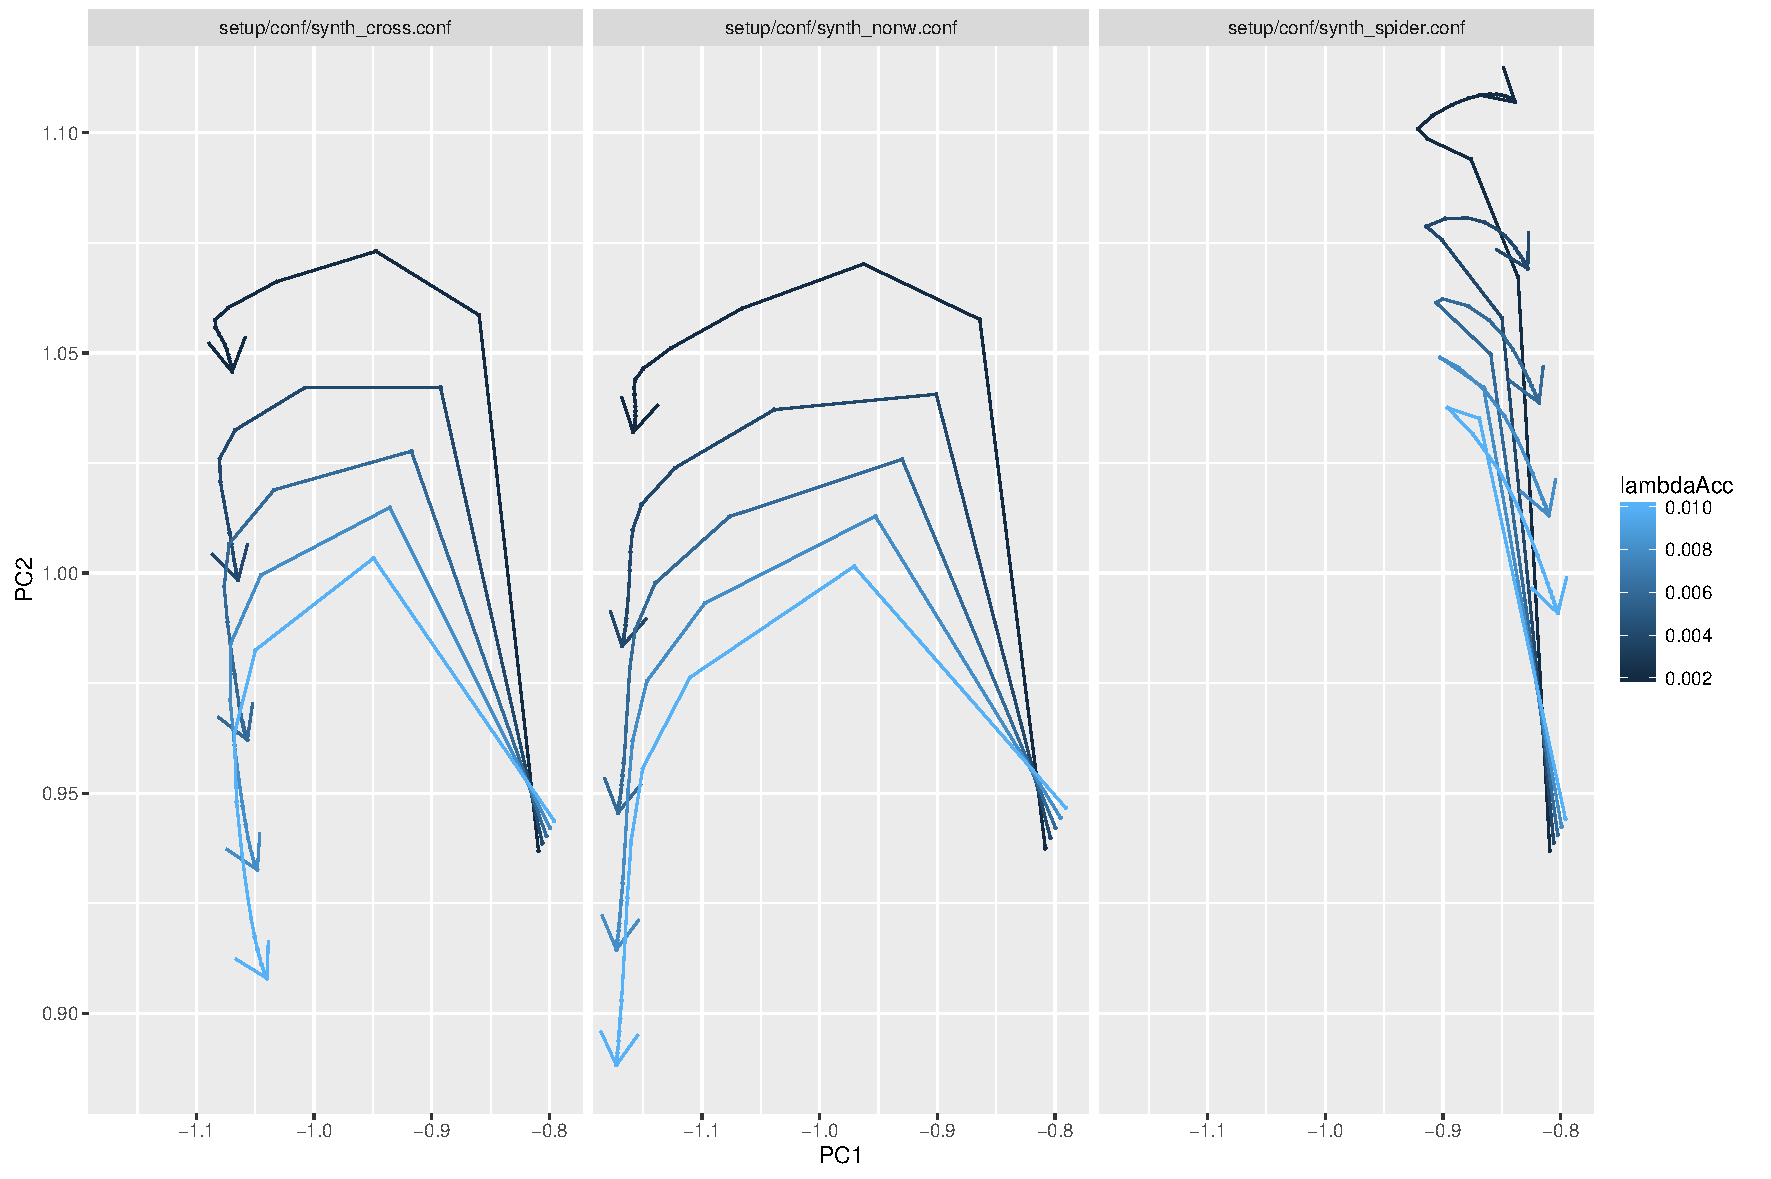
\includegraphics[width=\linewidth]{Figures/Lutecia/morphoActiveTrajsvaryinglambda_betaDC1_euclpace6.pdf}
	%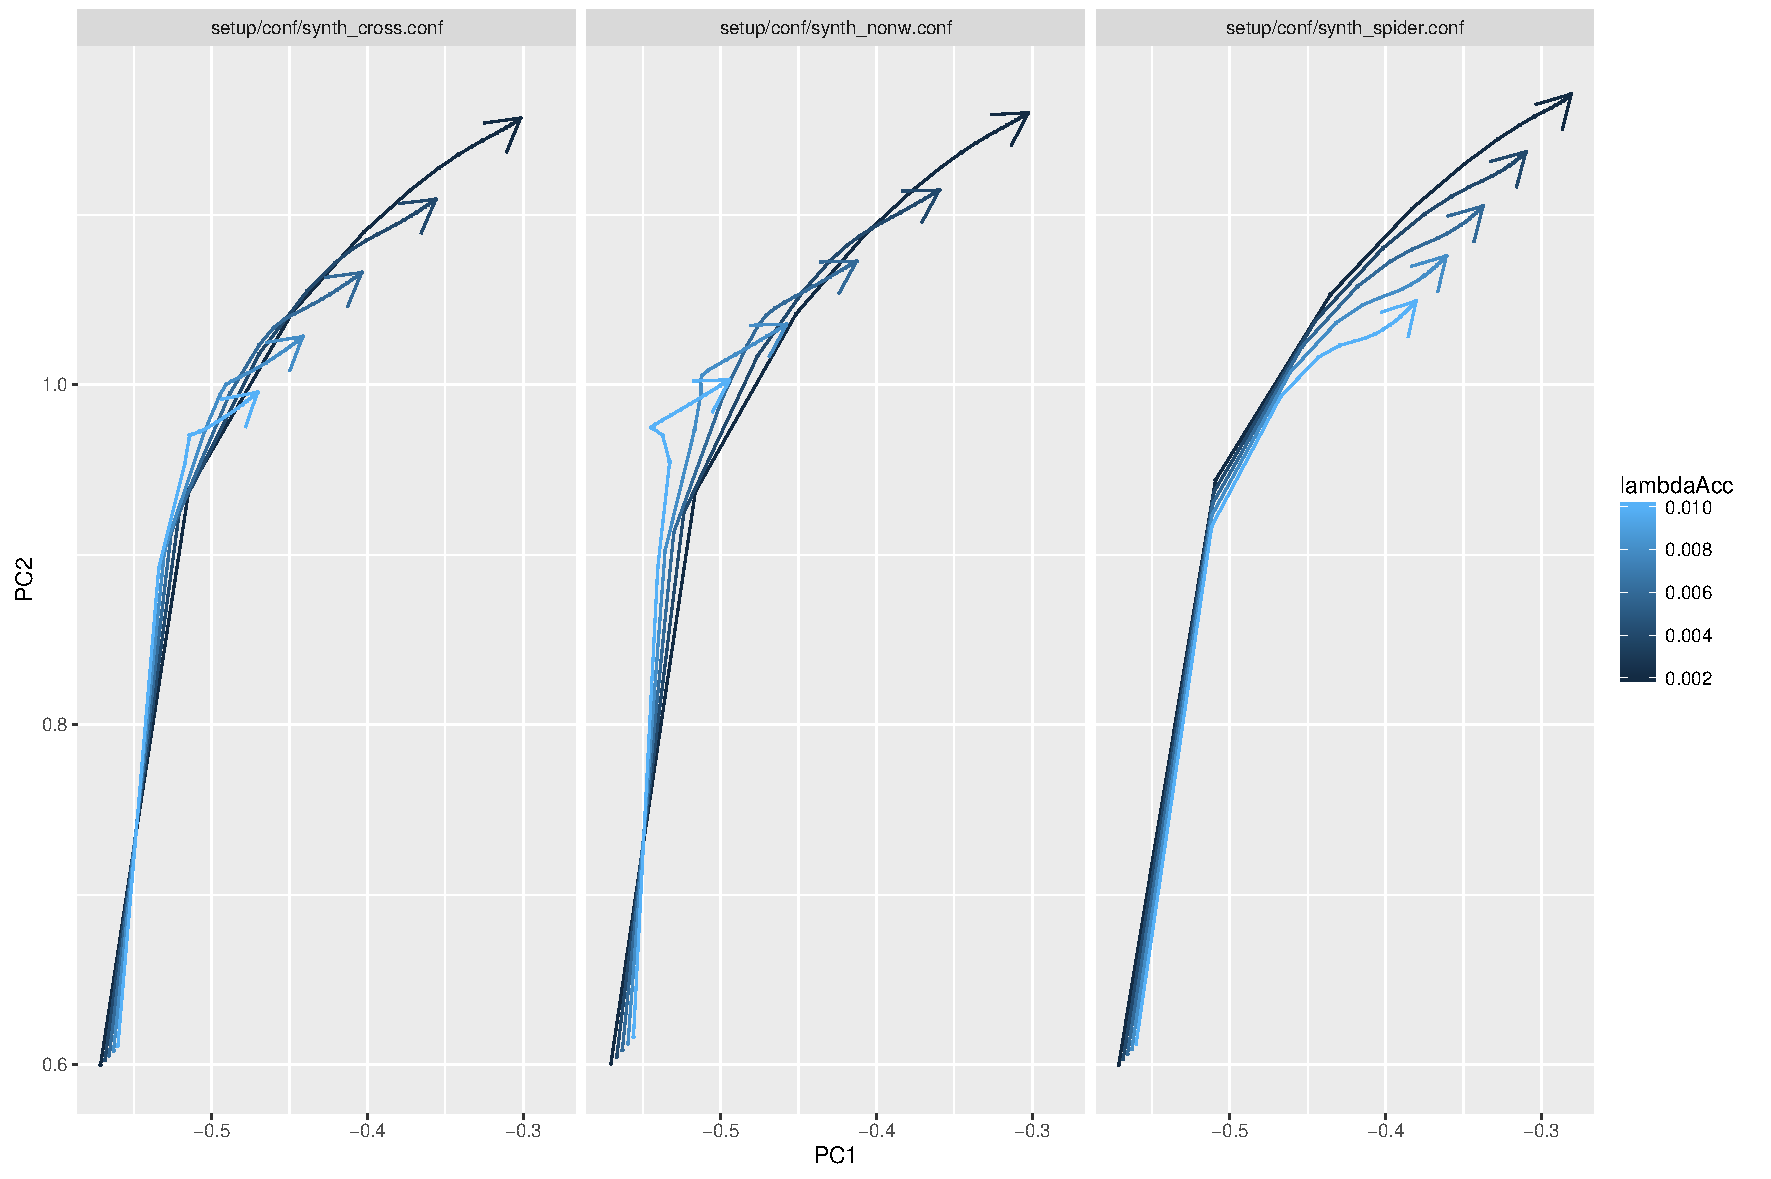
\includegraphics[width=\linewidth]{Figures/Lutecia/morphoActiveTrajsvaryinglambda_betaDC2_euclpace6.pdf}
	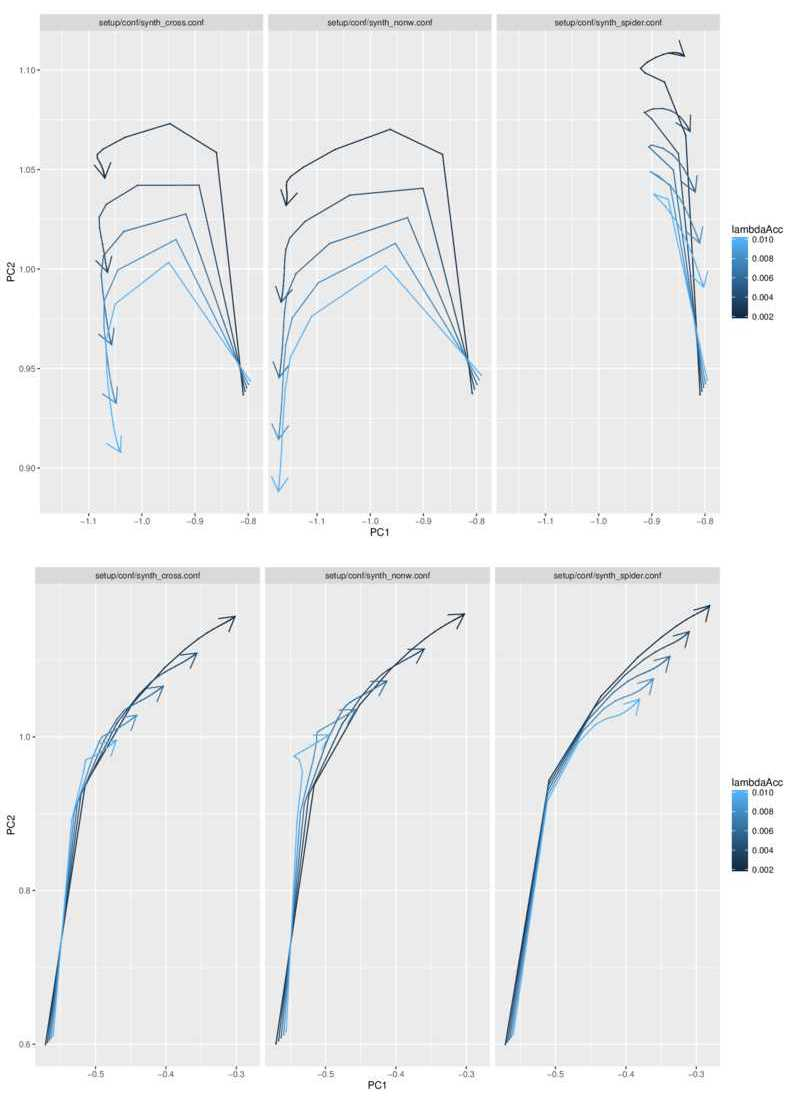
\includegraphics[width=\linewidth,height=0.9\textheight]{Figures/Final/A-lutecia-morphotrajs.jpg}
	\appcaption{\textbf{Morphological trajectories for the distribution of population.} We fix here $\gamma_A = 0.9$ and $\gamma_E = 0.6$. (\textit{Top}) Trajectories in the space $(PC_1,PC_2)$ for $\beta = 1$, with variable $\lambda$ (color), and for three different network configurations (columns): cross network, no network, cross network with branches (spider). (\textit{Bottom}) Same plots, for $\beta = 2$.\label{fig:app:lutecia:morphotrajs}}{\textbf{Trajectoires morphologiques pour la distribution de population.} On fixe ici $\gamma_A = 0.9$ et $\gamma_E = 0.6$. (\textit{Haut}) Trajectoires dans l'espace $(PC_1,PC_2)$ pour $\beta = 1$, avec $\lambda$ variable (couleur), et pour trois configurations de réseau différentes (colonnes) : réseau en croix, pas de réseau, réseau en croix avec ramifications (spider). (\textit{Bas}) Mêmes graphes, pour $\beta = 2$.\label{fig:app:lutecia:morphotrajs}}
\end{figure}
%%%%%%%%%%%%%%


\bpar{
The Fig.~\ref{fig:app:lutecia:morphosens} gives the value of $PC1_$ for the final configuration on all the space of explored parameters. We thus observe the variability of forms (here in terms of dispersion) as a function of all parameters: for example, for large $\beta$ values, complex diagrams emerge. For low $\beta$ values, we have a diagonal privileged for dispersion within concentrated configurations.
}{
La Fig.~\ref{fig:app:lutecia:morphosens} donne la valeur de $PC_1$ pour la configuration finale sur l'ensemble de l'espace des paramètres exploré. Nous constatons ainsi la variabilité des formes (ici en termes de dispersion) en fonction de l'ensemble des paramètres : par exemple, pour des grandes valeurs de $\beta$, des diagrammes complexes émergent. Pour les faibles valeurs de $\beta$, on a une diagonale privilégiée pour la dispersion au sein de configurations concentrées.
}


%%%%%%%%%%%%%%
\begin{figure}
	%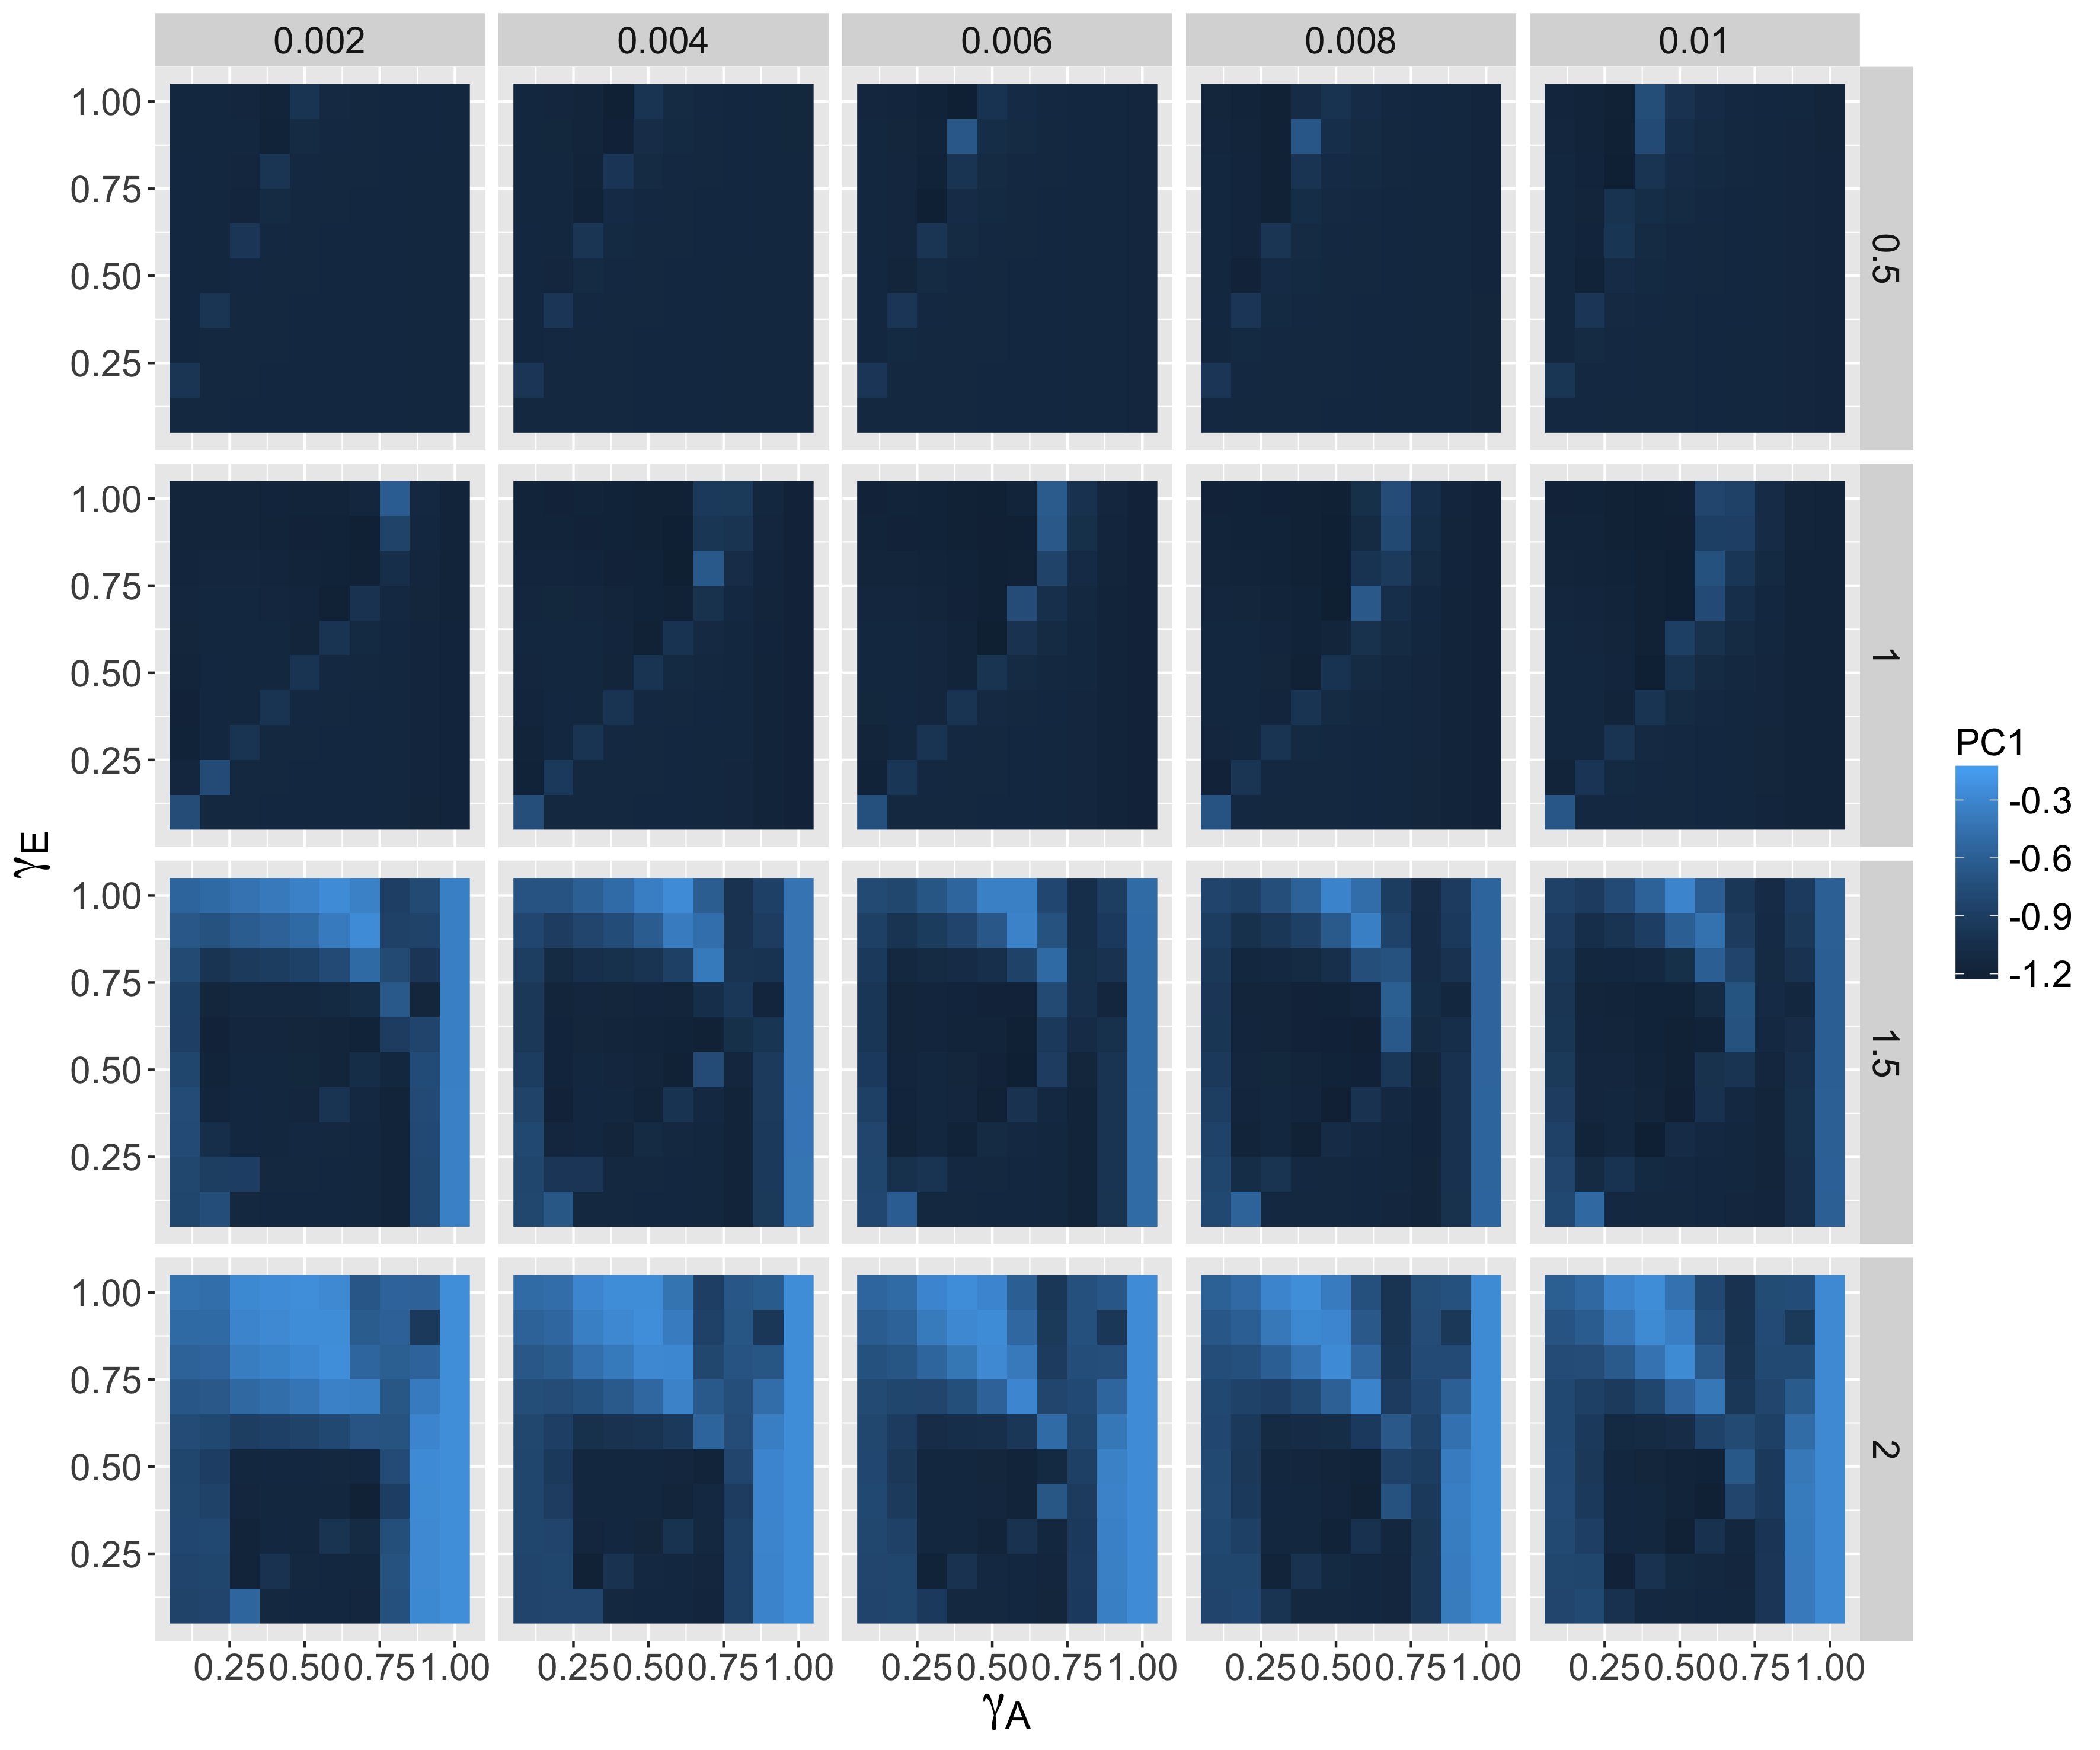
\includegraphics[width=\linewidth]{Figures/Lutecia/PC1_synth_nonw_euclpace6.png}
	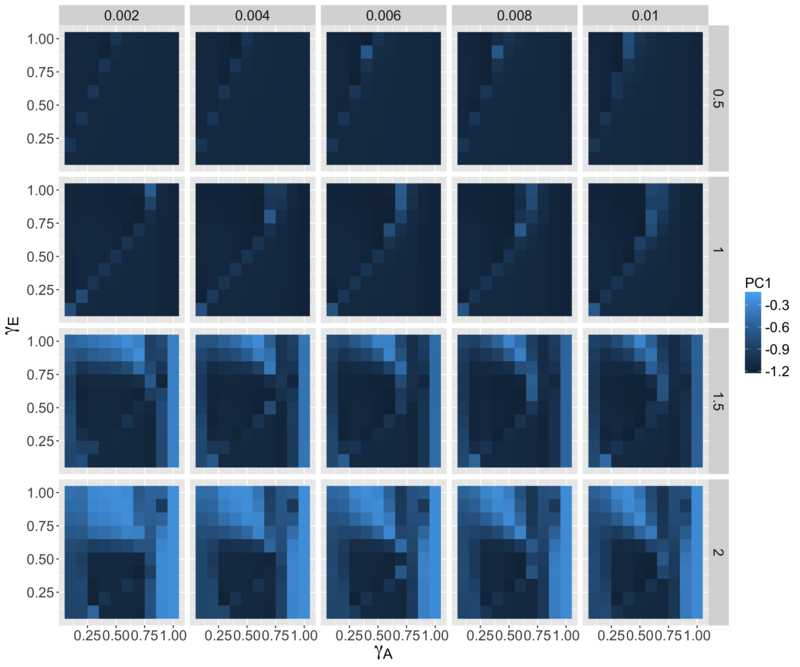
\includegraphics[width=\linewidth]{Figures/Final/A-lutecia-morphosens.jpg}
	\appcaption{\textbf{Sensitivity of the urban form.} For the distribution of populations, without initial network, value of $PC_1$ as a function of $(\gamma_A,\gamma_E)$, with variable $\lambda$ (columns) and variable $\beta$ (rows).\label{fig:app:lutecia:morphosens}}{\textbf{Sensibilité de la forme urbaine.} Pour la distribution des populations, sans réseau initial, valeur de $PC_1$ en fonction de $(\gamma_A,\gamma_E)$, avec $\lambda$ variable (colonnes) et $\beta$ variable (lignes).\label{fig:app:lutecia:morphosens}}
\end{figure}
%%%%%%%%%%%%%%



\bpar{
Finally, in order to understand the influence of parameters on total mobility within a complete trajectory, we study in Fig.~\ref{fig:app:lutecia:ludiff} the cumulated variation of actives given by $\tilde{\Delta} = \sum_t \sum_k \left|\Delta A_k (t)\right|$. We see that high values of $\gamma_A$, for a high $\beta$, allow to minimize the total quantity of relocalization, which have a very low dependence in $\gamma_E$. It is therefore possible to optimize, even at fixed $\alpha$, the total quantity of urban sprawl.
}{
Enfin, afin de comprendre l'influence des paramètres sur la mobilité totale au cours d'une trajectoire complète, nous étudions en Fig.~\ref{fig:app:lutecia:ludiff} la variation cumulée des actifs donnée par $\tilde{\Delta} = \sum_t \sum_k \left|\Delta A_k (t)\right|$. On voit que des valeurs fortes de $\gamma_A$, pour $\beta$ élevé, permettent de minimiser la quantité totale de relocalisation, qui ne dépend que très faiblement de $\gamma_E$. Il est ainsi possible d'optimiser, même à $\alpha$ fixé, la quantité totale d'étalement urbain.
}


%%%%%%%%%%%%%%
\begin{figure}
	%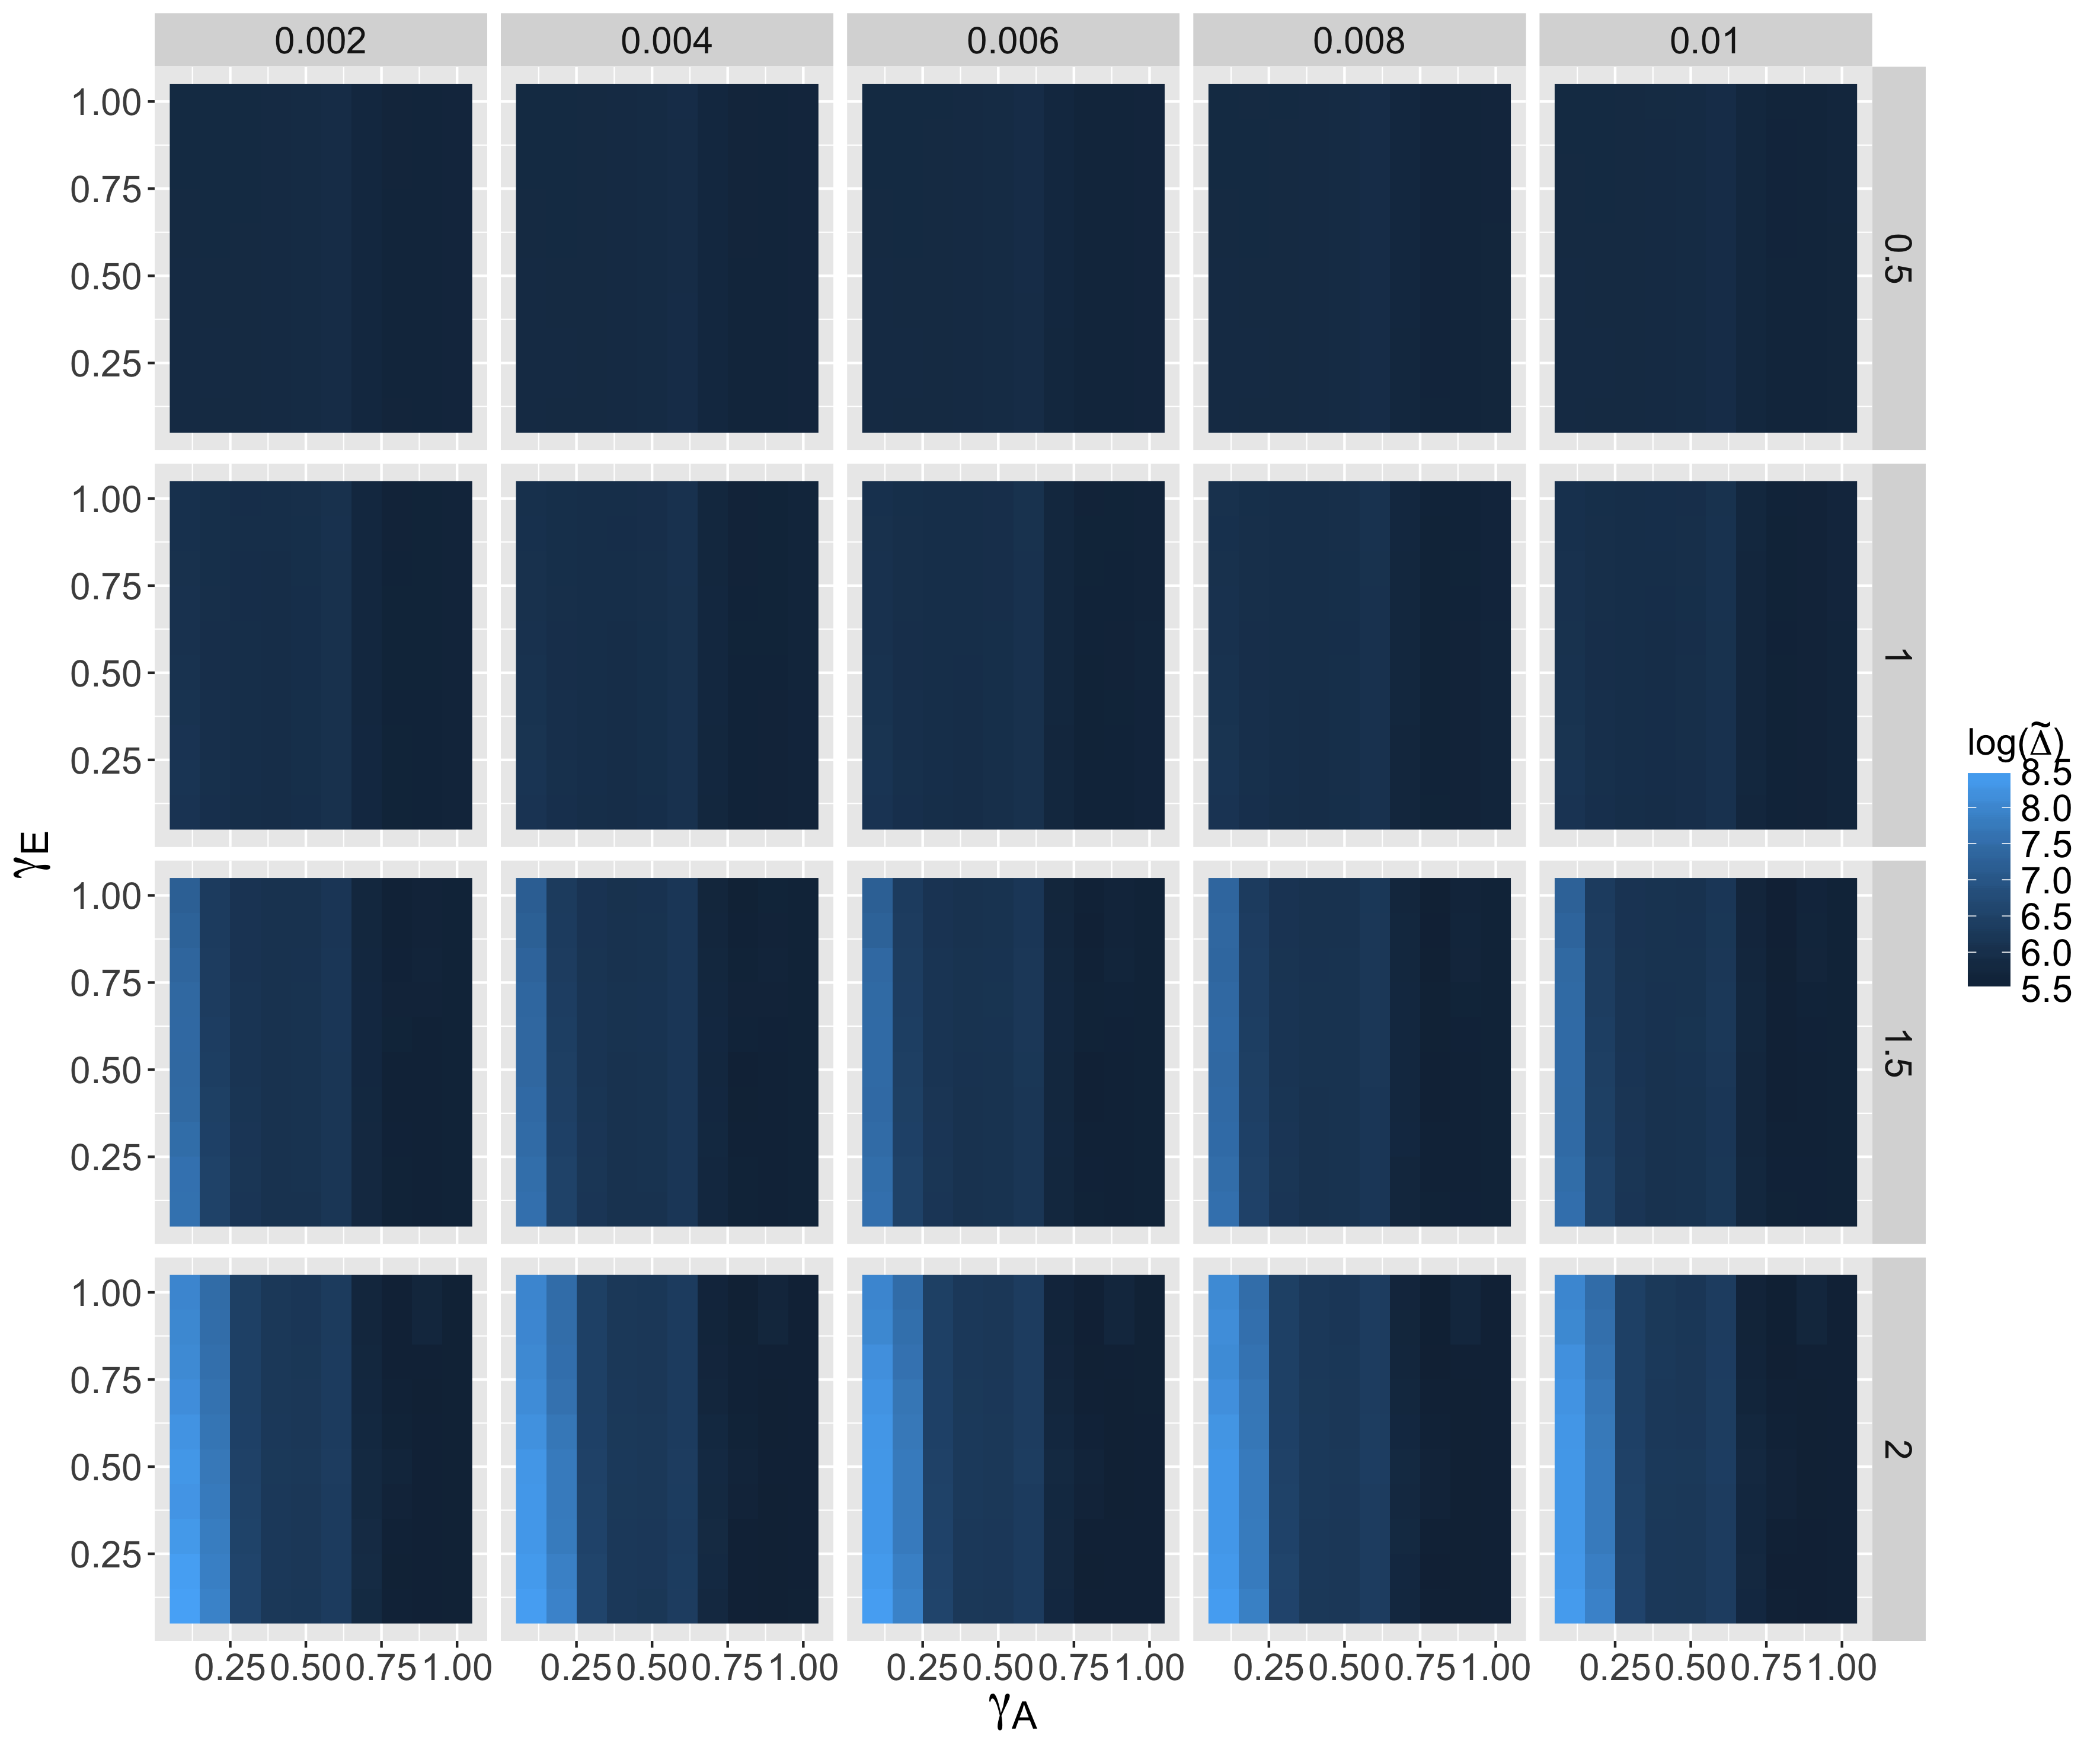
\includegraphics[width=\linewidth]{Figures/Lutecia/rdiffact_synth_nonw_euclpace6.png}
	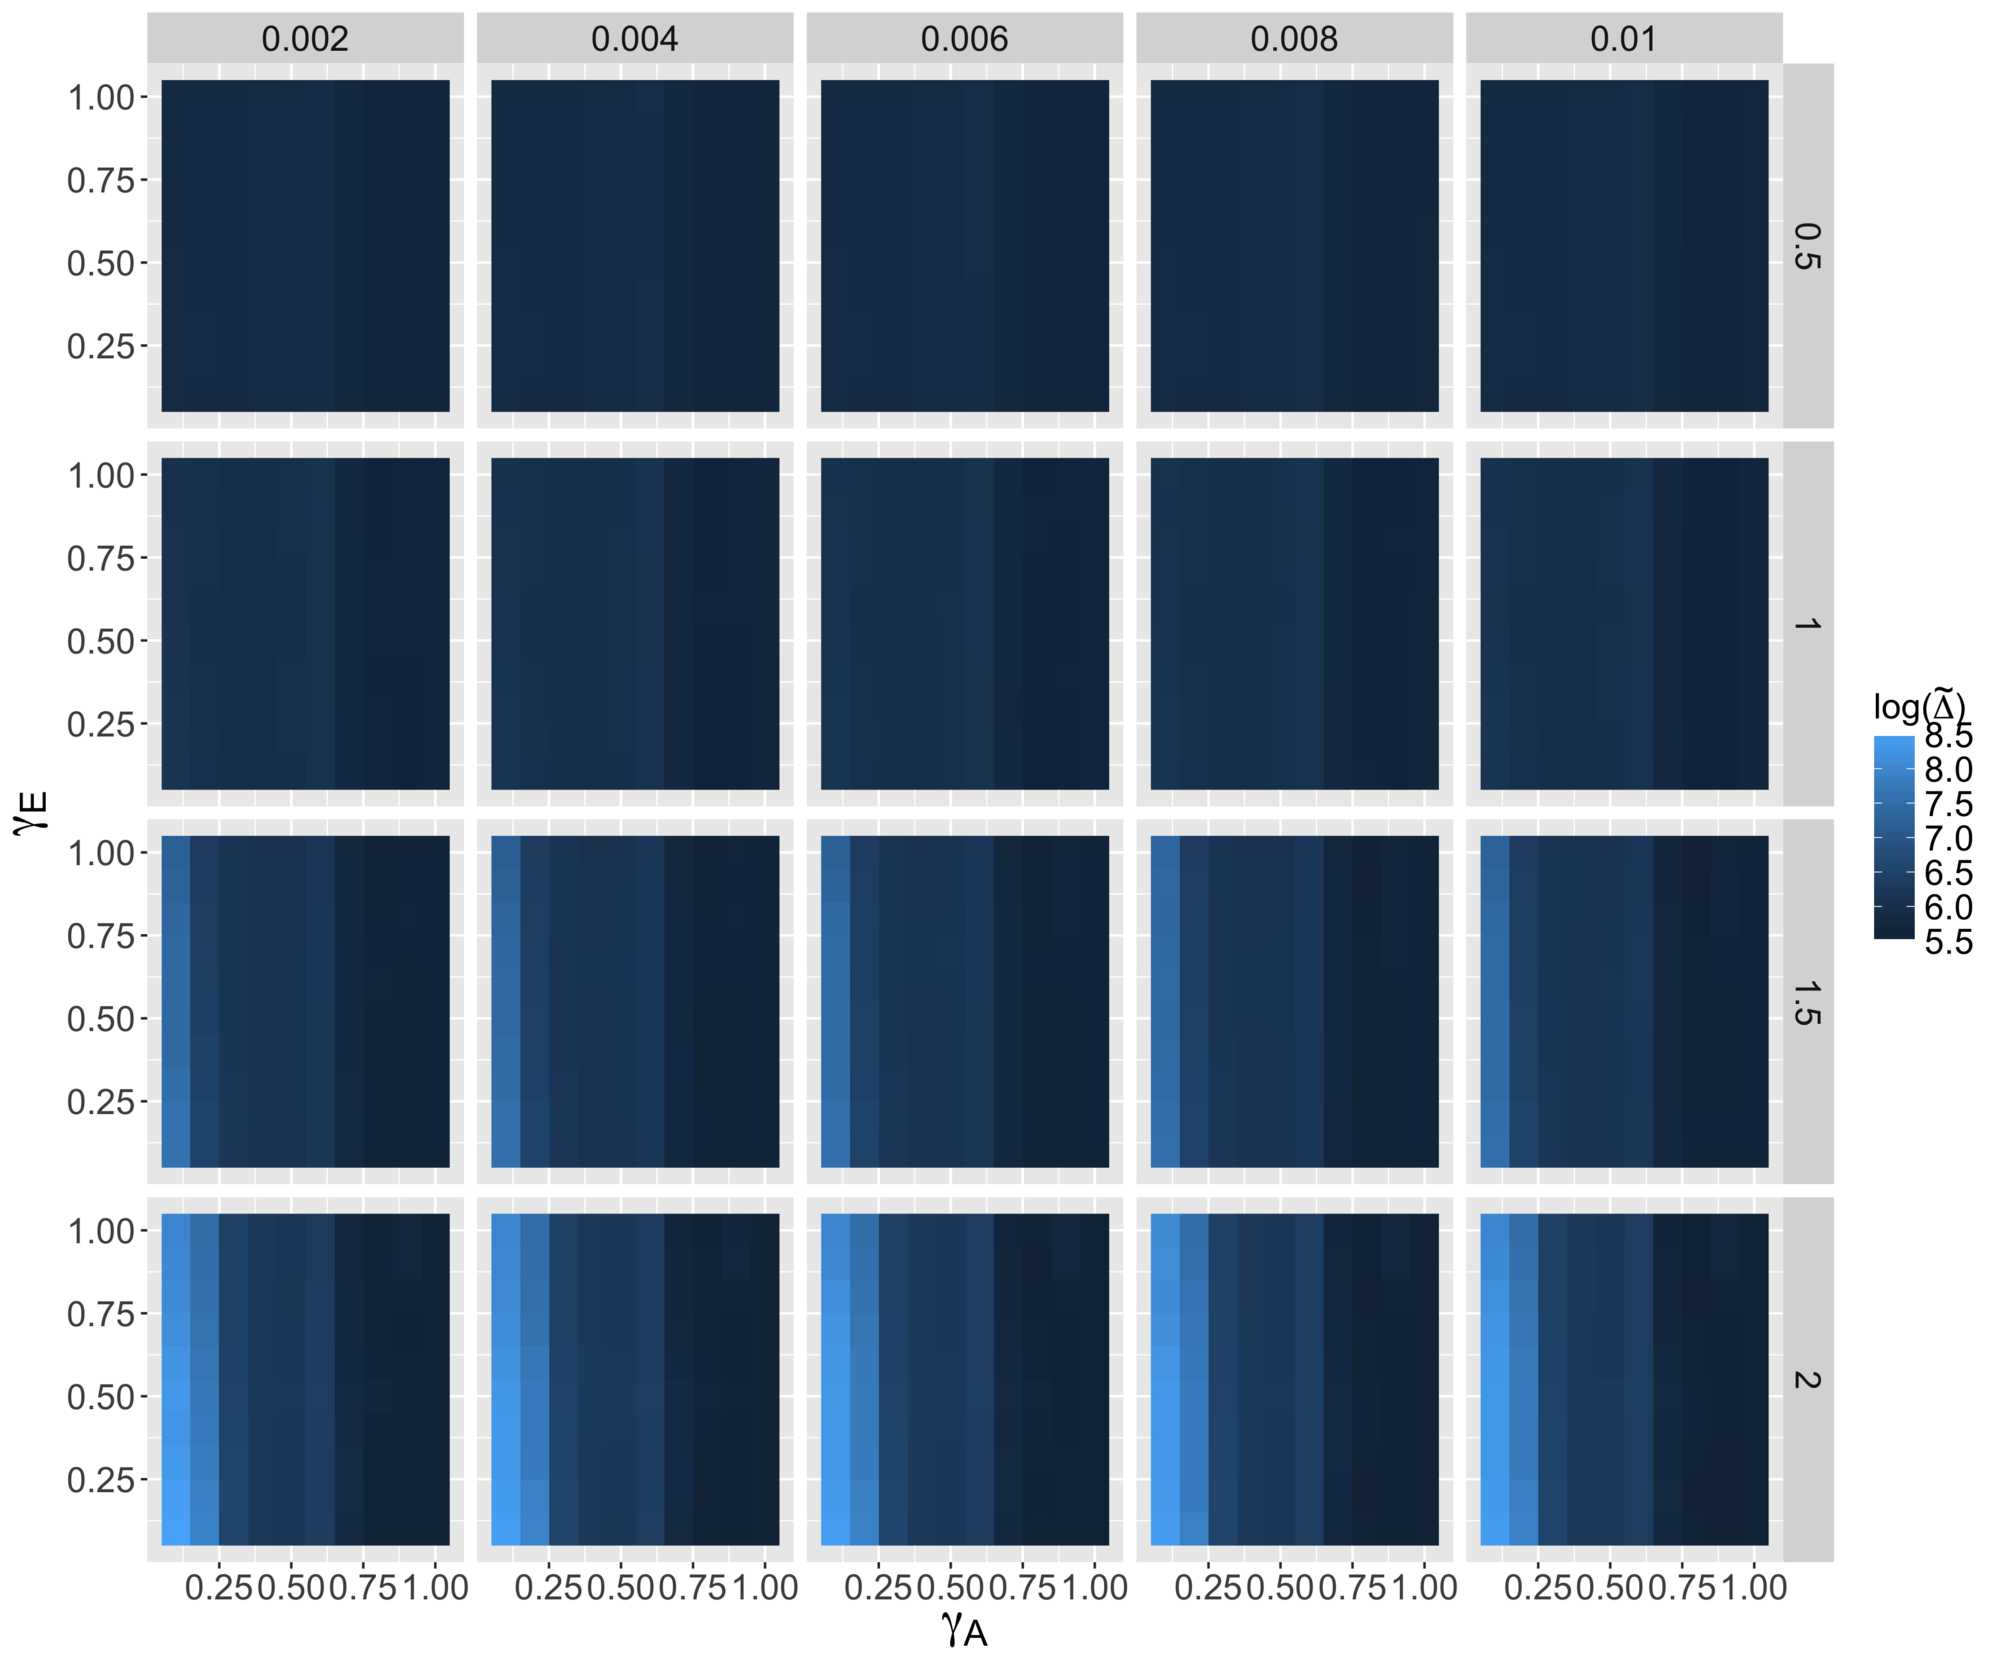
\includegraphics[width=\linewidth]{Figures/Final/A-lutecia-ludiff.jpg}
	\appcaption{\textbf{Cumulated variability of urban configurations.} Value of $\ln\tilde{\Delta}$, without initial network, as a function of $(\gamma_A,\gamma_E)$, with variable $\lambda$ (columns) and variable $\beta$ (rows).\label{fig:app:lutecia:ludiff}}{\textbf{Variabilité cumulée des configurations urbaines.} Valeur de $\ln\tilde{\Delta}$, sans réseau initial, en fonction de $(\gamma_A,\gamma_E)$, avec $\lambda$ variable (colonnes) et $\beta$ variable (lignes).\label{fig:app:lutecia:ludiff}}
\end{figure}
%%%%%%%%%%%%%%





%%%%%%%%%%%%%%%%%%%%%%%
\subsection{Transportation model}{Modèle de transport}


\bpar{
We did not take into account transportation flows in our implementation of the model, assuming that the constructed infrastructures have a sufficient capacity to be significantly not sensitive to congestion.
}{
Nous n'avons pas pris en compte les flux de transport dans notre implémentation du modèle, supposant que les infrastructures construites sont de capacités suffisantes pour ne pas être significativement sensibles à la congestion.
}


\bpar{
For the computation of flows between cells, the operation is the following: flows $\phi_{ij}$ are computed by a solving on $p_i,q_j$ through a fixed point method (Furness algorithm), of the system of gravity flows:
}{
Pour le calcul des flux entre cellules, l'opération est la suivante : les flux $\phi_{ij}$ sont calculés par résolution sur $p_i,q_j$ par une méthode de point fixe (algorithme de Furness), du système des flux gravitaires :
}


\[
\begin{cases}
\phi_{ij} = p_i q_j A_i E_j \exp{\left(-\lambda_{tr} d_{ij}\right)}\\
\sum_k \phi_{kj} = E_j\\
\sum_k \phi_{ik} = A_i\\
p_i = \frac{1}{\sum_k{q_k E_k \exp{(-\lambda_{tr}d_{ik})}}}\\
q_j = \frac{1}{\sum_k{p_k A_k \exp{(-\lambda_{tr}d_{kj})}}} 
\end{cases}
\]

\bpar{
where $\lambda_{tr}$ is a parameter giving the spatial reach of daily flows. The iteration of the last two equations rapidly converges starting from equal weights, by maintaining at each stage normalized weights.
}{
où $\lambda_{tr}$ est un paramètre donnant la portée spatiale des flux journaliers. L'itération des deux dernières équations converge rapidement à partir de poids égaux, en maintenant à chaque étape des poids normalisés.
}

\bpar{
In order to implement the stage of flows distribution within the network, when flows between cells are known, we should for example determine flows of the Static User Equilibrium with an appropriated algorithm. An assignment by shortest paths is implemented with the computation of flows in the model, but we deactivate this process in order to simplify the study of the model.
}{
Pour implémenter l'étape de distribution des flux dans le réseau, une fois les flux entre cellules connus, il faudrait par exemple déterminer les flux de l'Equilibre Utilisateur Statique avec un algorithme approprié. Une affectation par plus courts chemins est implémentée avec le calcul des flux dans le modèle, mais nous désactivons ce processus pour simplifier l'étude du modèle.
}


\bpar{
Congestion can be computed as a ratio to capacity, as $c/c_{max}$ if $c$ is the flow and $c_{max}$ the capacity. The speed is obtained with a BPR function of the form $v(c) = v_0 \left(1 - \frac{c}{c_max}\right)^{\gamma_c}$. Our configuration os equivalent to assuming an infinite capacity $c_{max} = \infty$.
}{
La congestion peut être calculée comme un rapport à la capacité, comme $c/c_{max}$ si $c$ est le flux et $c_{max}$ la capacité. La vitesse est obtenue par une fonction BPR sous la forme $v(c) = v_0 \left(1 - \frac{c}{c_{max}}\right)^{\gamma_c}$. Notre configuration revient à supposer une capacité infinie $c_{max} = \infty$.
}


\subsection{Probabilities to cooperate}{Probabilités de coopération}


\bpar{
The equilibrium assumption implies that conditional expectancies of each player are equal given their two choices, i.e. that
}{
L'hypothèse d'équilibre implique que les espérances conditionnelles de chaque joueur sont égales étant donné leur deux choix, i.e. que 
}
\[
\Eb{U_i|S_i=C} = \Eb{U_i|S_i=NC}
\] 

\bpar{
It is indeed equivalent in that case to maximize $\Eb{U_i}$ as a function of $p_i$, since by conditioning we have $\Eb{U_i} = p_i \Eb{U_i|S_i = C} + (1 - p_i) \Eb{U_i|S_i = NC}$,
}{
Cela revient en effet dans ce cas à maximiser $\Eb{U_i}$ par rapport à $p_i$, puisque en conditionnant on a $\Eb{U_i} = p_i \Eb{U_i|S_i = C} + (1 - p_i) \Eb{U_i|S_i = NC}$, et donc $\frac{\partial \Eb{U_i}}{\partial p_i} = \Eb{U_i|S_i = C} - \Eb{U_i| S_i = NC}$.
}

On a alors

\[
\Eb{U_i|S_i=C} = p_{1-i} U_i(S_i=C,S_{1-i}=C) + (1- p_{1-i}) U_i (S_i=C,S_{1-i}=NC)
\]

et donc 

\begin{equation*}
\hspace{-1cm}
\begin{split}
	p_{1-i} & U_i(S_i=C,S_{1-i}=C) + (1- p_{1-i}) U_i (S_i=C,S_{1-i}=NC) \\
	& = p_{1-i} U_i(S_i=NC,S_{1-i}=C) + (1- p_{1-i}) U_i (S_i=NC,S_{1-i}=NC)
\end{split}
\end{equation*}

ce qui donne

\[
p_{1-i} = - \frac{U_i(C,NC) - U_i(NC,NC)}{\left(U_i(C,C) - U_i(NC,C)\right) - \left(U_i(C,NC) - U_i(NC,NC)\right)}
\]

En substituant les expressions des utilités à partir de la matrice de gain, on obtient l'expression de $p_i$ en fonction du coût de collaboration $J$ et de la différence des différentiels d'accessibilité.


\subsubsection{Discrete choice coordination}{Coordination par choix discrets}


Pour déterminer la probabilité de coopération dans le cas des choix discrets, il s'agit de résoudre $f(p_i) = 0$ avec
\[
f(x) = \frac{1}{1+\exp\left[-\beta_{DC}\frac{\Delta_i}{1 + \exp(-\beta_{DC}(x \Delta_{1-i} - J))} - J\right]} - x
\]
où nous avons noté $\Delta_i = \Delta X_{i}(Z^{\star}_{C}) - \Delta X_{\bar{i}}(Z^{\star}_{i})$.

On a immédiatement $f(0) > 0 $ et $f(1) < 0$ et $f$ est continue, il existe donc toujours une solution $x\in [0,1]$ par le théorème des valeurs intermédiaires.

Concernant l'unicité, il est possible de la montrer sous certaines conditions. Un calcul de $\frac{\partial f}{\partial x}$ donne 
\[
\frac{\partial f}{\partial x} = 2 (\cosh u(x) - 1) + \beta^2 \Delta_i \Delta_{1-i} \frac{\exp(-\beta_{DC}(x \Delta_{1-i} - J))}{(1 + \exp(-\beta_{DC}(x \Delta_{1-i} - J)))^2}
\]

où $u(x) = -\beta_{DC} (\frac{\Delta_i}{1 + \exp(-\beta_{DC}(x \Delta_{1-i} - J))} - J)$.

Comme $\cosh u \geq 1$, on a $\frac{\partial f}{\partial x} > 0$ si $\Delta_i \Delta_{1-i} > 0$. La fonction est dans ce cas strictement croissante et on a une unique solution.

En pratique, la solution est déterminée par algorithme de Brent, avec les bornes $[0,1]$ et une tolérance de $0.01$.


%%%%%%%%%%%%%%%%%%%%%%%
\subsection{Implementation details}{Détails d'implémentation}


\paragraph{Distance Matrix}{Matrice des distances}

\bpar{
Distance via network are updated in a dynamical programming fashion for efficiency purposes (because of the numerous network updates), the following way :
\begin{enumerate}
\item Euclidian distance matrix $d(i,j)$ is computed analytically
%\item Network shortest paths between network intersections (rasterized network) updated in a dynamic way (addition of new paths and update or change of old paths if needed when a link is added), correspondance between network patches and closest intersection also updated dynamically ; $O(N_{inters}^3)$
%\item Weak component clusters and distance between clusters updated ; $O(N_{nw}^2)$
%\item Network distances between network patches updated, through the heuristic of only minimal connexions between clusters ; $O(N_{nw}^2)$
%\item Effective distances (taking paces/congestion into account) updated as minimum between euclidian time and \[\min_{C,C'}{d(i,C)+d_{nw}(p_C(i),p_C'(j))+d(C',j)}\], complexity in $O(N_{clusters}^2\cdot N^2)$ (Approximated with $\min_C$ only in the implementation, consistent within the interaction ranges $\sim$ 5 patches taken in the model). 
\end{enumerate}
}{
La matrice des distances est mise à jour de manière dynamique pour des questions de rapidité d'execution (vu le nombre de mises à jour du réseau), de la façon suivante :
\begin{enumerate}
	\item La matrice de distance euclidienne $d(i,j)$ est calculée analytiquement
	\item Les plus courts chemins entre les intersections des liens (entre les cellules du réseau raster correspondant) sont mis à jour de manière dynamique (étape de complexité $O(N_{inters}^3$) :
	\begin{itemize}
		\item Pour chaque nouvelle intersection, les plus courts chemins vers l'ensemble des autres intersections sont calculés par l'ancienne matrice et le nouveau lien.
		\item Pour l'ensemble des anciens plus courts chemins, ils sont mis à jour si besoin après vérification des éventuels raccourcis par le nouveau lien.
		\item La correspondance entre les cellules quelconques du réseau et les intersections est mise à jour.
	\end{itemize}
	\item Les composantes connexes et les distances entre celles-ci sont mises à jour (complexité en $O(N_{nw}^2)$)
	\item Les distances par le réseau entre les cellules du réseau sont mises à jour, avec l'heuristique des connexions minimales uniquement (un lien unique le plus court entre chaque cluster) (complexité en $O(N_{nw}^2)$)
	\item Les distances effectives entre l'ensemble des cellules (prenant la vitesse et la congestion en compte si celle-ci est implémentée) sont calculées comme le minimum entre la distance euclidienne et 
	\[\min_{C,C'}{d(i,C)+d_{nw}(p_C(i),p_C'(j))+d(C',j)}\]
	dont nous prenons une approximation avec $\min_C$ uniquement dans l'implémentation, ce qui est consistant avec les portées d'interaction relativement faibles considérées. La complexité est en $O(N_{clusters}^2\cdot N^2)$.
\end{enumerate}
}


\paragraph{Network growth}{Croissance du réseau}


Les infrastructures potentielles, au nombre de $N_I$ lors de la recherche heuristique d'une infrastructure optimale, sont tirées aléatoirement parmi l'ensemble des infrastructures possibles ayant une extrémité au centre d'une cellule. Si l'extrémité est à une distance inférieure à un seuil $\theta_I$ d'un lien déjà existant du réseau, celle-ci est remplacée par sa projection sur le lien correspondant. Il s'agit de l'étape d'accrochage permettant d'obtenir un réseau de forme raisonnable localement. En cohérence avec la représentation raster du réseau, nous prenons $\theta_I = 1$, ce qui correspond à la taille d'une cellule. 






%%%%%%%%%%%%%%%%%%
\subsection{Setup}{Initialisation}


\subsubsection{Synthetic setup}{Initialisation synthétique}

\bpar{
This section describes the setup in the case of synthetic configurations of MCR.
}{
Nous décrivons ici les détails de l'initialisation synthétique.
}


\bpar{
Initial distribution of Actives and Employments is done around governance centers at positions $\vec{x}_i$ using exponential kernels by
}{
Les distributions initiales des actifs et des emplois dans la configuration synthétique sont pris autour des centres de gouvernance (maires) aux positions $\vec{x}_i$ avec des noyaux exponentiels par
}

\[
A(\vec{x}) = A_{max} \cdot \exp{\left(\frac{\norm{\vec{x}-\vec{x}_i}}{r_A}\right)} ; 
E(\vec{x}) = E_{max} \cdot \exp{\left(\frac{\norm{\vec{x}-\vec{x}_i}}{r_E}\right)}
\]



\subsubsection{Setup on a real configuration}{Initialisation sur configuration réelle}

Nous montrons en Fig.~\ref{fig:app:lutecia:realsetup} la population et les réseaux sur lesquels les expériences sur données réelles sont menées : à usage du sol fixe,
\begin{itemize}
	\item une expérience sans réseau initial, et avec pour réseau cible de calibration le réseau de 2010 ;
	\item une expérience avec le réseau initial de 2010, et pour réseau cible le réseau planifié.
\end{itemize} 


%%%%%%%%%%%%%
\begin{figure}
	%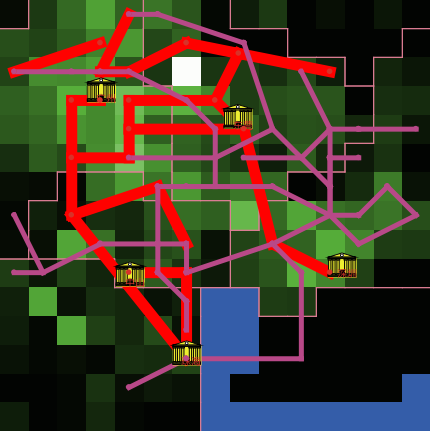
\includegraphics[width=\linewidth]{Figures/Lutecia/ex_real_filesetup.png}
	%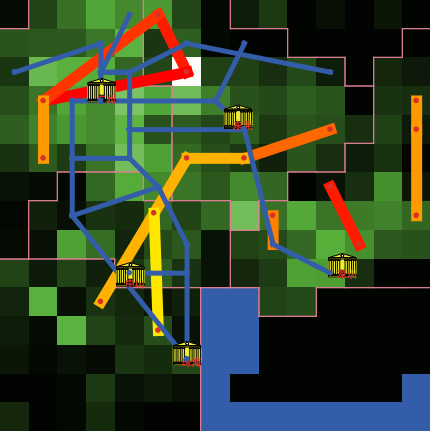
\includegraphics[width=\linewidth]{Figures/Lutecia/realnonw_nolu.png}
	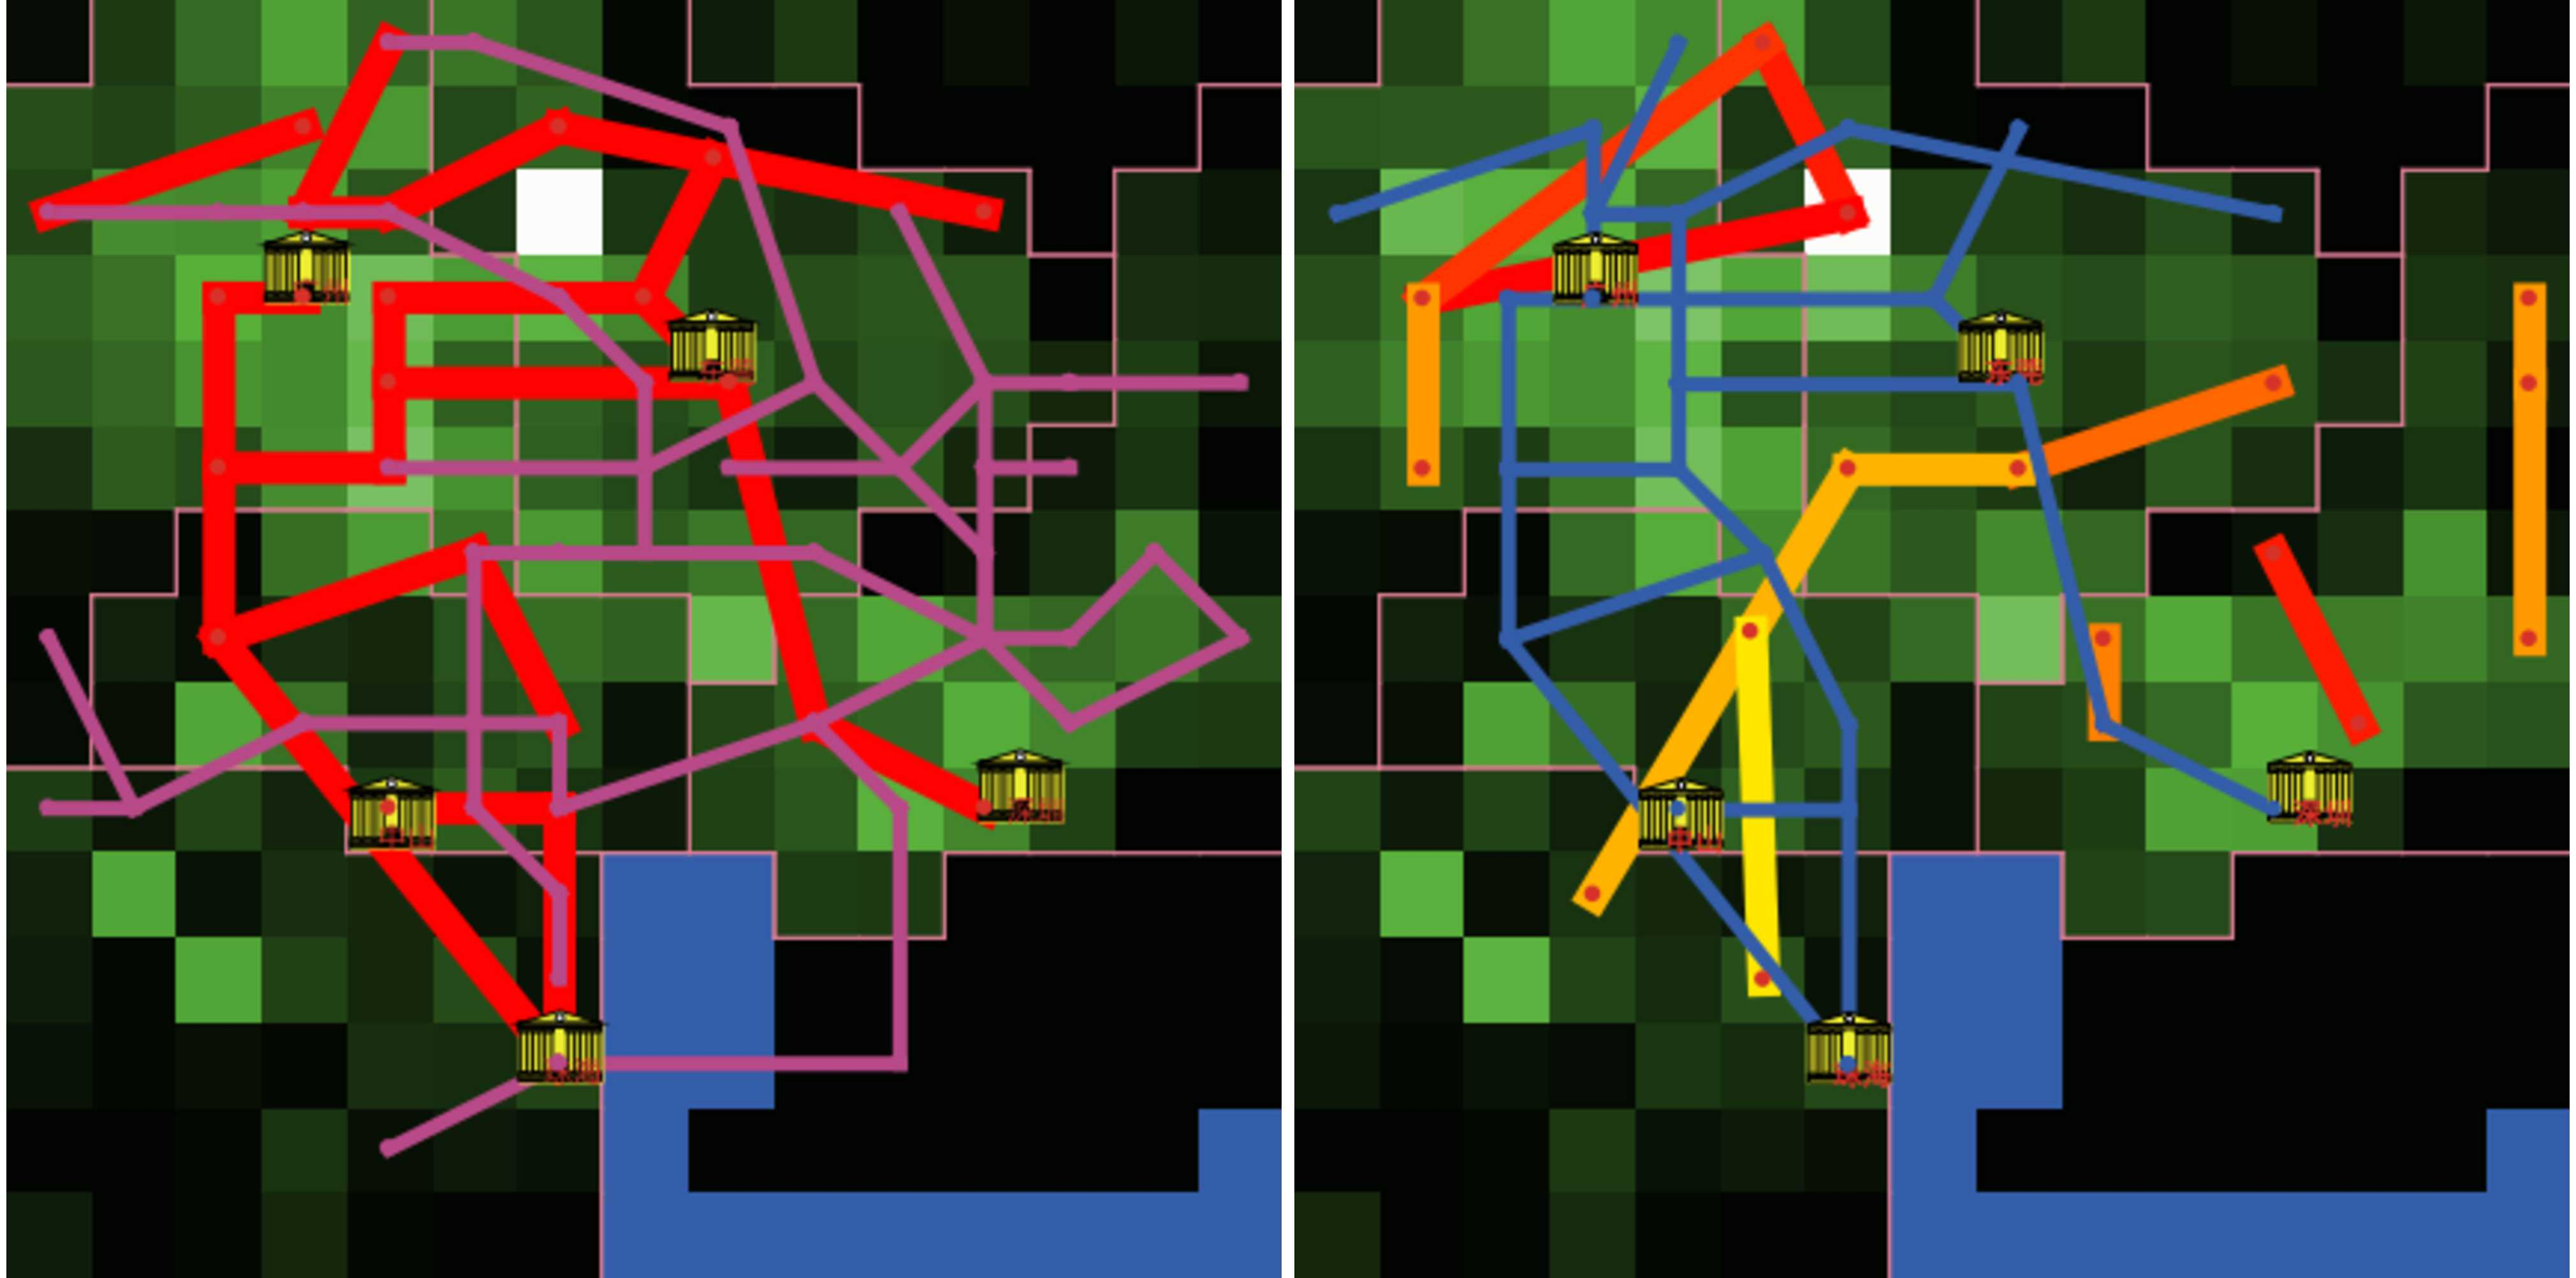
\includegraphics[width=\linewidth]{Figures/Final/A-lutecia-realsetup.jpg}
	\appcaption{\textbf{Setup on real data used for model application.}\label{fig:app:lutecia:realsetup}}{\textbf{Initialisation sur données réelles utilisée lors de l'application.} Pour des raisons de performances computationnelle, le nombre de cellules est ici diminué par rapport à l'illustration en texte principal. (\textit{Gauche}) Réseaux à l'initialisation, en rouge le réseau initial correspondant au réseau en 2010, en violet fin le réseau cible pour la calibration, correspondant au réseau planifié. (\textit{Droite}) Résultat obtenu avec $\alpha = 0$ à $t_f = 11$ après une initialisation sans réseau ; en bleu le réseau cible, qui correspond au réseau de 2010.\label{fig:app:lutecia:realsetup}}
\end{figure}
%%%%%%%%%%%%%

 









